\documentclass[fleqn,usenatbib,useAMS]{mnras}
\usepackage{amsmath}	% Advanced maths commands
\usepackage{txfonts}
\usepackage[T1]{fontenc}
\usepackage{ae,aecompl}
\usepackage{graphicx,color}	% Including figure files
\usepackage{amssymb}	% Extra maths symbols
\usepackage{amsbsy}
\usepackage[normalem]{ulem}
\usepackage{mathrsfs,bm,xspace}
\newcommand{\bcdot}{\ensuremath{%
  \mathchoice%
   {\mskip\thinmuskip\lower0.2ex\hbox{\scalebox{1.5}{$\cdot$}}\mskip\thinmuskip}}%
   {\mskip\thinmuskip\lower0.2ex\hbox{\scalebox{1.5}{$\cdot$}}\mskip\thinmuskip}%        
   {\lower0.3ex\hbox{\scalebox{1.2}{$\cdot$}}}%  
   {\lower0.3ex\hbox{\scalebox{1.2}{$\cdot$}}}%
}

% --- macros --- %
\newcommand{\Mstream}{{\it M-streaming}\xspace}
\newcommand{\Mflatturb}{{\it M-turbulence}\xspace}
\newcommand{\Mprimary}{{\it M-primaries}\xspace}

\renewcommand{\vec}{\ensuremath{\mathbfit}}
\newcommand{\dd}{\mathrm{d}}
\newcommand{\Vph}{\varv_\mathrm{ph}}
\newcommand{\mug}{\umu G}
\newcommand{\RH}{R_\rmn{RH}}
\newcommand{\bvel}{\ensuremath{\boldsymbol{\varv}}}
\newcommand{\bnabla}{\ensuremath{\boldsymbol{\nabla}}}
\newcommand\eb{\epsilon_\rmn{B}}
\newcommand{\dps}{\displaystyle}
\newcommand{\p}{\rmn{p}}
\newcommand{\kB}{k_{\rmn{B}}}
\newcommand{\eps}{\varepsilon}

%\voffset.6in 

\definecolor{mygreen}{rgb}{0.,0.5,0.}
\def\del#1{{}}
%\def\del#1{{\bf (DELETED TEXT)}}
\def\C#1{{\bf #1}}
\def\AP2#1{{\bf  AP2: #1}}
\def\AP#1{{\bf {\color{blue} AP: #1}}}
\def\SPO#1{{\bf {\color{red} SPO: #1}}}
\def\CP#1{{\bf {\color{mygreen} CP: #1}}}

\title[Origin of Seed Electrons]{Turbulence and Particle Acceleration in Giant Radio Halos: the Origin of Seed Electrons}  

\author[A. Pinzke, S. Peng Oh and C. Pfrommer] 
{Anders Pinzke$^{1,2}$\thanks{apinzke@fysik.su.se (AP); peng@physics.ucsb.edu (SPO); christoph.pfrommer@h-its.org (CP)}, S. Peng Oh$^{3}$ and Christoph Pfrommer$^{4}$\footnotemark[1]\\
$^{1}$The Oskar Klein Centre for Cosmoparticle Physics, Stockholm University, AlbaNova University Center, SE - 106 91
  Stockholm, Sweden\\
$^{2}$Dark Cosmology Center, University of Copenhagen,
  Juliane Maries Vej 30, DK-2100 Copenhagen, Denmark\\
  $^{3}$University of California - Santa Barbara,
  Department of Physics, CA 93106-9530, USA\\
$^{4}$Heidelberg Institute for Theoretical Studies
  (HITS), Schloss-Wolfsbrunnenweg 35, 69118 Heidelberg, Germany}

\begin{document}
\pagerange{\pageref{firstpage}--\pageref{lastpage}} \pubyear{2015}
\maketitle
\label{firstpage}

%\date{\today}

%\pacs{98.65.Cw, 98.70.Sa, 95.85.Bh, 95.30.Qd, 95.30.Cq, 94.05.Lk, 94.05.Pt}

 
\begin{abstract}
  About one third of X-ray-luminous clusters show smooth, unpolarized
  radio emission on $\sim$Mpc scales, known as giant radio halos. One
  promising model for radio halos is Fermi II acceleration of seed
  relativistic electrons by compressible turbulence in the
  intracluster medium (ICM); Coulomb losses prohibit acceleration from
  the thermal pool. However, the origin of seed electrons has never
  been fully explored. Here, we integrate the Fokker-Planck equation
  of the cosmic ray (CR) electron and proton distributions in
  cosmological simulations of cluster formation. For standard
  assumptions, structure formation shocks lead to a seed electron
  population which produces too centrally concentrated radio
  emission. Instead, we present three plausible scenarios for the seed
  CRs that each can reproduce the spatially flat radio emission
  observed in the Coma cluster. (1) The CR proton-to-electron
  acceleration efficiency $K_\rmn{ep} \sim 0.1$ is assumed to be
  larger than in our Galaxy ($K_\rmn{ep} \sim 10^{-2}$), due to the
  magnetic geometry at the shock. The resulting primary electrons
  dominate the radio emission, which is more extended in comparison to
  radio emission from secondary electrons that result from hadronic CR
  interactions in the ICM. (2) CR protons may stream at the Alfv{\'e}n
  speed to the cluster outskirts when the ICM is relatively
  quiescent. A spatially flat CR proton distribution develops and
  produces the required population of secondary seed electrons. (3)
  The ratio of injected turbulent-to-thermal energy density increases
  significantly with radius, as seen in cosmological simulations. This
  generates a flat radio profile when CRs are reaccelerated even if
  the seed population of CRs is steep with radius. These competing
  non-trivial solutions provide incisive probes of non thermal
  processes in the high-$\beta$ ICM.
\end{abstract} 

%% --- keywords --- %
%\begin{keywords}
%  magnetic fields, cosmic rays, radiation mechanisms: non-thermal, elementary
%  particles, galaxies: cluster: general, Galaxy: fundamental parameters
%\end{keywords}
%%\maketitle


% --- section: Introduction --- %
\section{Introduction}
About one third of X-ray-luminous clusters show smooth, unpolarized
radio emission on $\sim$Mpc scales, known as giant radio halos (RHs)
\citep{2014IJMPD..2330007B}. They appear only in disturbed, merging
clusters and the RH luminosity correlates with the X-ray luminosity
\citep{2001A&A...369..441G,2012A&ARv..20...54F} and the Compton
$y$-parameter \citep{2012MNRAS.421L.112B,2013A&A...554A.140P}. The RHs
show that CR electrons and magnetic fields permeate a large volume
fraction of the intra-cluster medium (ICM). The dominant CR source,
given the smoothness and enormous extent of RHs, is thought to be
structure formation shocks \citep{miniati01,pfrommer08}. At the same
time, plasma processes, the origin of magnetic fields and particle
acceleration in a turbulent, high-$\beta$ plasma like the ICM are not
well understood. Radio halos thus provide an incisive probe of
non-thermal processes in the ICM.

There have been two competing models proposed to explain RHs.  The
radio emitting electrons in the ``hadronic model'' are produced in
inelastic (hadronic) CR proton interactions with protons of the
ambient thermal ICM, which generates pions that eventually decay into
electrons and positrons, depending of the charge of the initial pion
(\citealp{1980ApJ...239L..93D,1999APh....12..169B,2001ApJ...562..233M,
  2004A&A...413...17P,2008MNRAS.385.1211P,ensslin11}). CR protons and
heavier nuclei may have been accelerated and injected into the ICM by
structure formation shocks, active galactic nuclei and galactic
winds. However, the strong bimodality that separates X-ray luminous
clusters into radio-active and radio-quite clusters (requiring a
fast switch on/off mechanism of the RH emission) and the very extended
RH emission at low frequencies in Coma (352~MHz) represent a major
challenge to this model class \citep{brunetti12,2014MNRAS.438..124Z}.

The alternative model for RHs is re-energization of seed suprathermal
electrons by Fermi II acceleration when ICM turbulence becomes
transonic during mergers
\citep{1987A&A...182...21S,1993ApJ...406..399G,2001MNRAS.320..365B,
  2004MNRAS.350.1174B,brunetti07,brunetti11,2015ApJ...800...60M}. Due
to the short radiative cooling time of high-energy relativistic
electrons, the cluster synchrotron emission quickly fades away after a
merger, which naturally explains the observed bimodality of RHs
\cite[see e.g.][]{2013MNRAS.429.3564D,2014MNRAS.443.3564D}.

However, there is a salient piece missing in the turbulent
reacceleration model. It relies heavily on the assumption of an
abundant, volume-filling population of seed suprathermal electrons;
direct Fermi II acceleration from the thermal pool is precluded by
strong Coulomb losses
\citep{2008ApJ...682..175P,2012ApJ...759..113C}. These seeds are
presumed to be either fossil CR electrons (CRes) accelerated by
diffusive shock acceleration (DSA) during structure formation
\citep{1999ApJ...520..529S}, or secondaries injected by hadronic
interaction of CR protons (CRps) with thermal protons
\citep{brunetti11}.

While analytic estimates have been made, there has been no ab initio
demonstration that structure formation can lead to the required
abundance of seed electrons with the correct spatial and spectral
characteristics. This is a non-trivial requirement: Coulomb cooling in
dense cluster cores is severe, and DSA fossil electrons may not
survive. On the other hand, for secondaries to constitute the seed
population, the CRp population required in the best-studied case of
the Coma cluster must have a very broad and flat (or even slightly
inverted) spatial profile \citep{brunetti12}, in contrast with the
thermal plasma whose energy density declines steeply with radius. In
Fig.~\ref{fig:Edens} we show that such a distribution is not predicted
by cosmological simulations \cite[see
  also][]{pinzke10,2014MNRAS.439.2662V}. If CRps are predominantly
advected with the cluster plasma, their distribution will be peaked
towards the cluster center and shows a similar characteristics as the
thermal plasma. As a consequence, the distribution of secondary
electrons and the resulting radio synchrotron emission is also peaked
since the hadronic reaction is a two-body scattering process. Hence,
the simulated emission falls short of the observed extended and flat
radio profile of the Coma cluster.

\begin{figure}
  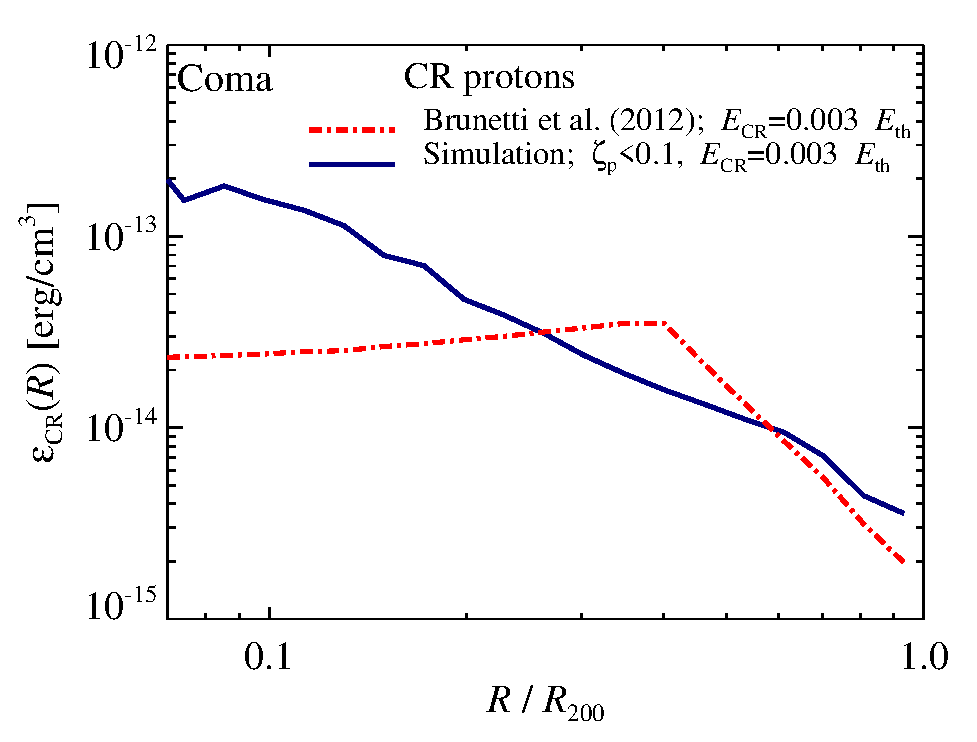
\includegraphics[width=1.0\columnwidth]{fCR.radius.coma.g72a.Rad14.2400p.z0.NL.xKR.eb23.eI067.DII.140.v6.eps}
  \caption{Spatial distribution of CRp energy density in the Coma
    cluster. The red dash-dotted line shows the required distribution
    of seed CRps that generate secondary electrons via proton-proton
    (p-p) collisions required to reproduce Coma radio brightness
    observations after Fermi-II reacceleration \citep{brunetti12}. The
    blue solid line shows the distribution of fossil CRps found in
    cosmological simulations, which disagrees with the required
    profile. To better compare the two models in this figure, we
    normalize the required distribution of CRps by fixing the total
    CRp energy $E_\rmn{CR}$ to 0.3 percent of the total thermal
    energy, consistent with observations
    \citep{2014ApJ...787...18A,2012ApJ...757..123A}.}
  \label{fig:Edens}
\end{figure}

Indeed, arriving at a seed population with the required
characteristics is highly constraining, and has the potential to teach
us much about the origin of CRps/CRes in clusters.  In this work, we
use our hydrodynamical zoom simulations of galaxy clusters in a
cosmological setting to follow the distribution functions of seed
populations for CRps and CRes, and integrate the Fokker-Planck
equation of CR transport along Lagrangian particle trajectories. We
model diffusive shock acceleration at structure formation shocks,
account for various loss processes of CRs, and -- most importantly --
model second-order Fermi acceleration by CR interactions with
magnetised turbulence.

However, we assume a simplified and stationary model for magnetic
fields and turbulence. We do not account for the time-varying energy
density in compressible waves, which are thought to be necessary for
the acceleration process \citep{brunetti07,brunetti11}, as the cluster
merger proceeds.  So our approach is orthogonal (and complementary) to
e.g., simulations of \citealp{2015ApJ...800...60M} that focus on the
time-dependent compressible turbulence while adopting a simplified
treatment of CR that does not follow the transport of the CR
distribution function. Our approach of parametrizing turbulence
enables us to vary parameters associated with the unknown continuation
of magneto-hydrodynamical (MHD) turbulence below the MHD scale and the
overall amplitude of compressible waves (that can in principle vary
depending on the details of a particular cluster merger).

In this paper we consider three new scenarios that
individually or combined can reproduce the observed radio profiles and
spectrum in the Coma cluster without violating gamma-ray constraints:
\begin{enumerate}
\item {\bf Model {\em M-primaries}.} If the acceleration efficiency of CRps is below
  about $0.1$~{\%} in weak (perpendicular) shocks and the ratio of injected
  electrons-to-protons $K_{\rmn{ep}} \sim 0.1$, this yields a dominant primary
  population with a flat spatial distribution, since primaries have a weaker
  density dependence than secondaries.
\item {\bf Model {\em M-streaming}.} Here, we account for streaming CRps that
  produce flat distributions of CRps in the ICM
  \citep{ensslin11,wiener13,2014MNRAS.438..124Z}, which also flattens the
  secondary electron distribution.
\item {\bf Model {\em M-turbulence}.} Here, we adopt a spatially
  flatter turbulent profile than what was adopted in \citet{brunetti12},
  but where seed CRps follow the steep profile that is suggested by
  structure formation simulations.
\end{enumerate}

To pursue these three possibilities further, we employ cosmological
simulations of CRs in clusters. In tandem with new insights from our
recent work on DSA generated fossil electrons \citep{pinzke13}, we
generate the first quantitative calculation of primary and secondary
seed electrons and compare to observations in the Coma cluster. For
the most part, we adopt parameters that are used in previous work,
including Fermi-II acceleration with models of turbulent spectra
\citep{brunetti07,brunetti11}, injection scale of turbulence
\citep{2015ApJ...800...60M}, the energy density of turbulence
\citep{2009ApJ...705.1129L,2010ApJ...725.1452S,2011A&A...529A..17V},
for CR acceleration in shocks \citep[][in particular $K_{\rmn{ep}}$
  and the acceleration efficiency]{pinzke13}, and for cosmological
simulations with CR physics \citep[][i.e., shock history,
  temperature profile, density profile, magnetic field
  profile]{pinzke10}. All these parameters are uncertain, and could
potentially change our predictions. We refer the reader to
section~\ref{sect:param_comp} for a first exploration of parameter
space, however we leave the detailed exploration of parameter space and
the interaction between free parameters to future work.


% --- section: Method --- %
\section{Cosmic ray transport}

The transport of relativistic electrons and protons across cosmic time
into galaxy clusters is a complex problem that depends on the velocity
field of the gas (and its thermodynamic properties such as density,
temperature, and pressure) as well as non-thermal processes
(turbulence, magnetic fields, fossil CRs). We use high resolution
galaxy cluster simulations to derive the thermal and fossil CR
properties \citep[shock accelerated primary CRes and CRps, as well as
  secondary CRes produced in p-p collisions,
  see][]{2007MNRAS.378..385P,pfrommer08,pinzke10,pinzke13}.


\subsection{Basic equations}
As previously noted, secondaries produced by shock accelerated CRp
have the wrong spatial profile to explain RH observations. Because
they arise from a two body process, they are too centrally
concentrated. They also produce $\gamma$-ray emission in excess of
Fermi-LAT upper limits
\citep{2012ApJ...757..123A,brunetti12,2014ApJ...787...18A}. However,
if CRps stream in the ICM, then their spatial profile could
potentially flatten sufficiently \citep{ensslin11,wiener13}. This
scenario is very attractive: it generates seed electrons with the
right spatial footprint, and by removing CRps from the core, obeys
gamma-ray constraints. Turbulence plays two opposing roles:
Alfv{\'e}nic turbulence damps waves generated by the CR streaming
instability \citep{yan02,farmer04}, thus reducing self-confinement;
but compressible fast modes scatter CRs directly. Turbulent damping is
still efficient for highly subsonic conditions \citep{wiener13}, while
we assume compressible fast modes to only provide effective spatial
confinement during the periods of transonic, highly super-Alfv{\'e}nic
($M_{\rm A} \sim 5$) turbulence associated with mergers. Thus, CRs can
stream out when the cluster is kinematically quiescent. Furthermore,
even Alfv{\'e}nic streaming timescales are relatively short
\cite[$\sim 0.1-0.5$ Gyr;][]{wiener13} compared to the timescale on
which the CRp population is built up. Based on these findings, we
adopt a toy model for our \Mstream scenario in which CR streaming
instantaneously produces flat CRp profiles. 

Given a seed population of CRs, we adopt essentially the same set of
plasma physics assumptions as the reacceleration model for RHs
\citep{brunetti07,brunetti11}. We solve the isotropic, gyro-phase
averaged Fokker-Planck equation (via a Crank-Nicholson scheme) for the
time evolution of the CRe distribution in the Lagrangian frame
\citep{brunetti07,brunetti11}:
\begin{eqnarray}
{{d f_{\rmn{e}}(p,t)}\over{d t}} &\!=&
\frac{\partial}{\partial p}
\left\{
f_{\rmn{e}}(p,t)\left[
\left|\frac{dp}{dt}\right|_{\rm Coul} 
+ \frac{p}{3}\left(\bnabla\bcdot \bvel\right)
+ \left|\frac{dp}{dt}\right|_{\rm rad}\right.\right.
\nonumber\\
&-& \left.\left.{1\over{p^2}}{{\partial }\over{\partial p}}\left(p^2 D_{pp}\right) 
\right]\right\} - \left(\bnabla\bcdot \bvel\right) f_{\rmn{e}}(p,t)
\nonumber\\
&+& {{\partial^2 }\over{\partial p^2}}
\left[
D_{pp} f_{\rmn{e}}(p,t) \right]+ Q_{\rmn{e}}\left[p,t;f_{\rmn{p}}(p,t)\right]   \, .
\label{elettroni}
\end{eqnarray}
Here $f_{\rmn{e}}$ is the one-dimensional distribution in position $x$
(suppressed for clarity), momentum $p$ and time $t$ (which is
normalized such that the number density is given by
$n_{\rmn{e}}(t)=\int d p f_{\rmn{e}}(p,t)$), $d/dt=\partial/\partial
t+\bvel\bcdot\bnabla$ is the Lagrangian derivative, $\bvel$ is the gas
velocity, $|dp/dt|$ represents Coulomb
\citep[Coul,][]{1972Phy....60..145G} and radiative
\citep[rad,][]{1979rpa..book.....R} losses, respectively,
\begin{eqnarray}
   \left|\frac{dp}{dt}\right|_{\rm Coul} &=& \frac{3\,\sigma_\rmn{T}\,n_e\,c}{2\, \beta^2}
  \left[\ln\left(\frac{m_e c^2 \beta \sqrt{\gamma-1}}{\hbar\,\omega_\rmn{plasma}}\right)\right.\nonumber \\
    &-&\ln(2)\left(\frac{\beta^2}{2}+\frac{1}{\gamma}\right)+\frac{1}{2}+
    \left.\left(\frac{\gamma-1}{4\gamma}\right)^2\right]\,, \\
  \left|\frac{dp}{dt}\right|_{\rm rad~} &=& \frac{4}{3}\frac{\sigma_\rmn{T}}{m_ec}\,
  \frac{p^2}{\beta}\,\left[1+\left(\frac{B}{B_\rmn{CMB}}\right)^2\right]\,.
\end{eqnarray}
Here $\beta = p/\sqrt{1+p^2}$ is the dimensionless velocity of CRs,
$\gamma=\sqrt{1+p^2}$ is the Lorentz factor of CRs,
$\omega_\rmn{plasma} = \sqrt{4\pi e^2 n_e / m_e}$ is the plasma
frequency, $n_e$ is the number density of free electrons, and
$\sigma_\rmn{T}= 8\pi e^4/3(m_e c^2)^2$ is the Thomson cross
section. The {\it rms} magnetic field strength is denoted by $B$ and
the equivalent field strength of the cosmic-microwave background is
given by $B_\rmn{CMB} = 3.24 (1 + z)^2\mu\rmn{G}$, where $z$ denotes
the redshift. In the peripheral cluster regions, where $B \ll
B_\rmn{CMB}$, the CRes loose virtually all their energy by means of
inverse Compton emission. $D_{pp}$ is the momentum space diffusion
coefficient (see Sects.~\ref{sec:dummy} and \ref{sec:reacc}), and
$Q_{\rmn{e}}$ denotes the injection rate of primary and secondary
electrons in the ICM (see Sect.~\ref{sec:cosmo_sim}). The first term
containing the expression $\bnabla\bcdot \bvel$ represents Fermi-I
acceleration and the second term of this form describes adiabatic
gains and losses.

During post-processing of our Coma-like cluster simulation, we solve
the Fokker-Planck equation over a redshift interval from $z=5$ to
0. The simulated cluster undergoes a major merger over the last
1-2~Gyrs that is thought to inject large turbulent eddies. Following
standard approaches
\citep{brunetti07,brunetti11,2004ApJ...614..757Y,2015ApJ...800...60M}
we assume that about one Gyr after core passage the fields have
decayed down to the smallest scales where reacceleration is most
efficient ($D_{pp}\sim k_\rmn{cut}$) and the radio halo turns on
shortly after. Note that the exact decay time of the turbulens is of
minor importance, since the thermal and CR quantities are very similar
a few 100 Myrs before and after $z=0$ where we have chosen to evaluate
the simulations. This delay naturally explains why giant radio halos
are only seen in a fraction of all merging clusters.

In all our calculations we assume that turbulent reacceleration
efficiently accelerates particles for $\tau_\rmn{cl}\sim650$~Myrs
(which is roughly the cascade time on which turbulence is damped) and
that during this turbulent phase CR streaming and spatial diffusion
can be neglected. In our \Mstream model, CR streaming and diffusion
are incorporated separately during kinematically quiescent times that
precede the merger. As a result, flat CRp profiles are produced on
relatively short timescales ($\sim 0.1-0.5$ Gyr). This allows us to
implicitly solve for CR streaming in our calculations, where we adopt
a toy model that enforce a flat CRp profile at all quiescent times
\citep{wiener13}. We assume that CRs cannot stream significantly past
perpendicular $B$-fields at the accretion shock, so that the total
number of CRs is conserved within the virial radius during the
streaming process. Finally, since streaming is much more efficient for
the CRps, we can ignore this effect for the CRes.

The time evolution of the spectral energy distribution of CRps,
$f_{\rmn{p}}$, is similarly given by:
\begin{eqnarray}
\lefteqn{
  {{d f_{\rmn{p}}(p,t)}\over{d t}} =
  {{\partial }\over{\partial p}}
  \left\{
  f_{\rmn{p}}(p,t)\left[ \left|{{dp}\over{dt}}\right|_{\rm Coul}
    + \frac{p}{3}\bnabla\bcdot \left(\bvel+\bvel_{\rmn{st}}\right)\right.\right.}
\nonumber\\
&&-\left.\left. {1\over{p^2}}{{\partial }\over{\partial p}}\left(p^2 D_{pp}\right)
\right]\right\} - f_{\rmn{p}}(p,t) \bnabla\bcdot \left(\bvel+\bvel_{\rmn{st}}\right) 
- \bvel_{\rmn{st}}\bcdot\bnabla f_{\rmn{p}}(p,t)
\nonumber\\
&&+\,\,\, {{\partial^2 }\over{\partial p^2}}
\left[ D_{pp} f_{\rmn{p}}(p,t) \right] - {{f_{\rmn{p}}(p,t)}\over{\tau_{\rm had}(p)}}
+ Q_{\rmn{p}}(p,t)\, ,
\label{eq:FP_p}
\end{eqnarray}
where $\bvel_{\rmn{st}}=-\varv_{\rmn{A}}\bnabla f_{\rmn{p}}/|\bnabla
f_{\rmn{p}}|$ is the streaming velocity in the isotropic transport
approximation, $\varv_{\rmn{A}}$ is the Alfv\'en speed,
and $Q_{\rmn{p}}(p,t)$ denotes the injection rate of shock accelerated
CRps as a function of momentum $p$ and time $t$ (see
Sect.~\ref{sec:cosmo_sim}). The timescale of
hadronic losses that produce pions via CRp collisions with thermal
protons of the ICM is given by 
\begin{eqnarray}
  \tau_{\rm had} = \left[c\,n_\rmn{th}\,\sigma^{+/-,0}(p)\right]^{-1}\,,
\end{eqnarray}
where we use the cross-section, $\sigma^{+/-,0}(p)$, given by the
fitting formula in \citep{1986ApJ...307...47D}.

\subsection{Dummy's guide} 
\label{sec:dummy} 

All of the physics of turbulent reacceleration is effectively encapsulated in the diffusion coefficient, which can be rewritten as \citep{2015ApJ...800...60M}:
\begin{equation}
D_{pp}(p) = \frac{ p^{2} \pi I_{\theta}(c_{s}/c)}{8 c} \langle k \rangle_{\mathcal{W}} \langle (\delta v_{\rm c})^{2} \rangle
\label{eqn:diffusion}
\end{equation}
\SPO{define $I_{\theta}(c_{s}/c)$ or explain its meaning in words and point to the definition provided in the next subsection.}
where
\begin{equation}
\langle k \rangle_{\mathcal{W}} = \frac{1}{\langle (\delta \varv_{\rm c})^{2} \rangle} \int_{k_{\rm L}}^{k_{\rm cut}} dk \, k \, \mathcal{W}(k) \approx \frac{s-1}{2-s} k_{\rm L} \left( \frac{k_{\rm cut}}{k_{\rm L}} \right)^{2-s} 
\end{equation}
is an energy-averaged wavenumber, $k_{\rm L}, k_{\rm cut}$ are the wavenumbers associated with the outer scale and the cutoff scale respectively, and we have assumed a total energy spectrum (both kinetic and potential energy, where the two are assumed to be in equipartition \citep{sarkar11}): 
\begin{equation}
\mathcal{W}(k) = \frac{(s-1) \langle (\delta \varv_{\rm c})^{2} \rangle}{k_{\rm L}} \left( \frac{k}{k_{\rm L}} \right)^{-s} 
\label{eqn:Wk}
\end{equation}
which defines the normalization $\langle (\delta \varv_{\rm c})^{2} \rangle$ (the subscript 'c' emphasizes that we specialize to compressive modes). Intuitively, we can understand the form of the the diffusion coefficient from the fact that for second-order Fermi acceleration, $\dot{p} \sim \Delta p/\tau \sim p\,\langle k c \rangle_{\mathcal{W}} (\delta \varv_{\rm c}/c)^{2}$, where $\tau^{-1} \sim \langle k c \rangle_{\mathcal{W}}$ is the energy averaged wave-particle interaction rate, and $\Delta p \sim p (\delta \varv_{\rm c}/c)^{2}$ is the typical momentum change during wave particle scattering. Thus: 
\begin{equation}
D_{pp} \sim p \dot{p} \sim p^{2} \langle k c \rangle_{\mathcal{W}} \left( \frac{\delta \varv_{\rm c}}{c} \right)^{2}. 
\end{equation}

Equations \ref{eqn:diffusion} and \ref{eqn:Wk} make the important aspects of turbulence clear: the energy in compressive modes $\langle (\delta v_{\rm c})^{2} \rangle$, the inner and outer scale ($k_{\rm cut}$ and $k_{\rm L}$), and the slope of the energy spectrum $s$. All of these can vary spatially and temporally. 

{\bf Energy in compressive modes} The total turbulence energy is typically $\sim 15-70\%$ of the thermal energy in a cluster \citep{vazza11}; it rises rapidly during a merger. The compressible component is $\sim 20-40\%$ of the total turbulent energy, and shows more rapid temporal variations compared to the compressible component \citep{2013ApJ...771..131B,2015ApJ...800...60M}. It is worth noting that in the subsonic regime of the solar wind \citep{yao11,howes12}, as well as most idealized calculations of turbulent driving, there is relatively little energy in the fast mode. For instance, the fiducial simulations of \citet{lynn14} with a sonic Mach number ${\mathcal M}_{\rm s} \sim 0.35$ and a plasma beta factor of $\beta \sim 1$ show that 50\%, 45\%, 5\% of the turbulent energy density is in the Alfv{\'e}n, slow, and fast modes, respectively. For higher $\beta \sim 3-10$, they find that the proportion of energy in fast modes drops to $< 1\%$, while the fraction of energy in the slow mode remains roughly the same. Similarly, \citet{kowal10} find that the fast mode is highly subdominant (see their Table 2); for the run most relevant to cluster conditions ${\mathcal M}_{\rm s} \sim 0.7, \beta \sim 10$, they find $\sim 42\%, 6\%$ of turbulent energy in slow and fast modes respectively. These simulations are roughly consistent with theoretical estimates of $U_{\rm fast}/U_{\rm slow} \sim {\mathcal M}_{\rm s}^{2}/{\mathcal M}_{\rm A}$ \citep{cho03}. By contrast, MHD simulations of galaxy clusters find a large fraction ($\sim 25$\%) of turbulent energy in fast modes \citep{2013ApJ...771..131B}. This is likely due to the compressive nature of turbulent driving (transonic infall and merger), whereas idealized simulations tend to use incompressible solenoidal driving and allow compressive fluctuations to develop on their own. 

In the high-$\beta$, subsonic conditions of the ICM, the Alfv{\'e}n/slow modes are exactly/approximately incompressible, and so the approximate identification of compressive modes with fast modes is valid. We therefore take $\sim 25\%$ of the turbulent energy density in compressive fast modes as a reasonable baseline estimate \citep{2013ApJ...771..131B,2015ApJ...800...60M}. If a large fraction of energy is in slow modes, then resonant broadening of wave-particle interactions can render slow modes an efficient acceleration mechanism \citep{lynn14}, as we discuss briefly in \S\ref{?}.

{\bf Slope of the energy spectrum $s$.} At large scales, turbulent motions are subsonic (${\mathcal M}_{\rm s} \sim 0.2-0.5$) but super-Alfv{\'e}nic (${\mathcal M}_{\rm A} \sim 5$). Thus, except in the case where motions are transonic and weak shocks become important, motions are fundamentally hydrodynamic and turbulence follows a Kolmogorov ($s=5/3$) spectrum. However, while the turbulent energy density $U_{\rm t} \propto l^{2/3}$ decreases at small scales, the magnetic energy density is scale-independent. Thus, at some scale $l_{\rm A} \sim l_{\rm o} {\mathcal M}_{\rm A}^{-3}$, where $U_{\rm turb} \sim U_{B}$, the magnetic field becomes dynamically important, and turbulence transitions to the MHD regime. Theory \citep{goldreich95,chandran05} and simulations \citep{cho03} show that in the MHD regime, the Alfv{\'e}n and slow modes have a shallower Kraichnan spectrum ($s=3/2$), with relatively little coupling between the incompressible and compressible modes \citep{cho02,cho03} -- though if weak shocks are important, $s=2$ may be more appropriate (see discussion below). 

Since the Kraichnan spectrum is critical in what follows, it is worthwhile taking a moment to recount the origin of the spectral slope $s$ and the cascade rate. In the magnetically dominated regime, two counterpropagating wave packets of scale $l$ interact on an Alfv{\'e}n time $\tau_{\rm A}=l/\varv_{\rm A}$, rather than the eddy turnover time $\tau_{\rm edd} = l/\varv_{\rm l}$. 
Since $\tau_{\rm A} \ll \tau_{\rm edd}$, each interaction results in a small velocity change $\delta \varv_{\rm l} \sim \varv_{\rm l} (\tau_{\rm A}/\tau_{\rm edd})$. If these changes behave like a random walk, the cascade time $\tau_{\rm l}$ it takes for an eddy to become non-linear ($\Delta \varv \sim \varv_{\rm l})$ and cascade to smaller scales is $\varv_{\rm l} \sim \delta \varv_{\rm l} (\tau_{\rm l}/\tau_{\rm A})^{1/2} \sim \varv_{\rm l} \tau_{\rm A}/\tau_{\rm edd} (\tau_{\rm l}/\tau_{\rm A})^{1/2}$, which we can solve to obtain the cascade time: 
\begin{equation}
\tau_{\rm l} \sim \left(\frac{\tau_{\rm edd}}{\tau_{\rm A}}\right)^{2} \tau_{\rm A} \sim \frac{l \varv_{\rm A}}{\varv_{\rm l}^{2}} 
\end{equation}
where we have implicitly assumed isotropy. This implies a dissipation rate $\epsilon \sim \varv_{\rm l}^{2}/\tau_{\rm l} \sim \varv_{\rm l}^{4}/(l \varv_{\rm A})$, or $\varv_{\rm l} \sim (\epsilon l \varv_{A})^{1/4}$. Thus, since $k E(k)\sim \varv_{\rm l}^{2}$, this gives a kinetic energy spectrum: 
\begin{equation}
E(k) \sim (\epsilon \varv_{\rm A})^{1/2} k^{-3/2}.
\end{equation}
 
Finally, if turbulence is transonic ($M_{\rm s} \sim {\mathcal O}(1)$), then compressible modes can dissipate in weak shocks, as seen in decompositions of the velocity field into solenoidal/compressible components both in idealized simulations \citep{kowal10,porter15}, and cosmological hydrodynamic simulations \citep{2015ApJ...800...60M}. The compressible component has a steep Burgers ($s=2$) spectrum. Burgers turbulence is distinct from other forms of turbulence in that it violates locality in k-space--i.e., power does not gradually cascade, but instead can directly jump from large to small scales via a network of weak shocks. Since the Fourier transform of a step function goes as $k^{-1}$, Burgers turbulence has a power spectrum of $P(k) \propto k^{-2}$. If we contrast the different velocity scalings: $\varv \propto l^{1/4}$ (Kraichnan), $\varv \propto l^{1/3}$ (Kolmogorov), $\varv \propto l^{1/2}$ (Burgers), we see that because of its dissipative nature, Burgers turbulence is the least efficient at transferring energy towards the small scales needed (since the wave particle interaction rate scales as $k$) for efficient acceleration. If Burgers turbulence dominates, then particle acceleration rates are too slow in the face of cooling processes to explain radio halos \citep{2015ApJ...800...60M}.

Given the lack of consensus on the fast mode spectrum, and the fact that turbulent reacceleration is not a viable explanation for radio halos if the spectrum is Burgers-like, we assume a Kraichnan spectrum. 

{\bf Inner and outer scale}

{\bf Timescales} 

{\bf Scaling solutions} Since the diffusion time is independent of energy (the so-call 'hard sphere' approximation), analytic solutions are possible. The steady state solution is a power-law with a cutoff above a characteristic momentum $p_{\rm eq}$, defined by $t_{\rm acc} \equiv t_{\rm cool} (p_{\rm eq})$ \citep{stawarz08}: 
\begin{equation}
n(p) \propto \left \{
\begin{array}{ll}
p^{-\sigma} & \quad \text{for} \quad p \ll p_{\text{eq}} \, , \\
p^2 {\rm e}^{-p/p_{\text{eq}}} & \quad \text{for} \quad p \sim p_{\text{eq}} \,.
\end{array}
\right.
\end{equation}
%
where $-\sigma = 1/2 - \sqrt{9/4 +
  t_\text{acc}/t_\text{esc}}$ asymptotically approaches $-1$
as $t_\text{acc}/t_\text{esc} \rightarrow 0$.


%%%Fast modes can become more important in highly supersonic turbulence, but this is not relevant to clusters. The magnetic energy density in fast modes scales as $\delta B^{2}_{\rm F} \sim \rho \delta v_{\rm F}^{2}/\beta$ (since magnetic restoring forces 


\subsection{Formalism for turbulent reacceleration}
\label{sec:reacc}

We incorporate momentum diffusion for electrons and protons via the
transit-time-damping (TTD) resonance with compressible MHD turbulence,
to model Fermi-II reacceleration \citep{brunetti07,brunetti11}. The
TTD resonance requires the wave frequency to obey the resonance
condition, $\omega=k_\parallel\varv_\parallel$, where $k_\parallel$
and $\varv_\parallel$ are the parallel (projected along the magnetic
field) wavenumber and particle velocity, respectively. This implies
that the particle transit time across the confining wave region
matches the wave period,
$\lambda_{\parallel}/\varv_{\parallel}=\tau_{\rmn{wave}}$. Note, the CRs'
gyroradius does not enter the resonance condition. Hence the CRs that
are in resonance with compressible waves experience Fermi-II
acceleration irrespectively of the length scale of the perturbation.

However, the resonance changes the component of the particle momentum
parallel to the mean magnetic field, which over time leads to
increasing anisotropy in the particle distribution that decreases the
efficiency of reacceleration with time. As in \citet{brunetti11}, we
assume that there exists a mechanism---such as the firehose
instability---that isotropizes the CR distribution function at the
gyroscale and on the reacceleration time scale, which ensures
sustained efficient reacceleration with time.

It can be shown that the particle pitch-angle averaged
momentum-diffusion coefficient of isotropic particles that couple to
fast magnetosonic modes via TTD resonance is \citep[][
  Eqn. 47]{brunetti07}:
\begin{eqnarray}
  D_{pp}(p,t) = \frac{\upi}{16} \frac{p^2}{\rho c}
  \left\langle\frac{\beta |B_k|^2}{16 \upi \,W}\right\rangle
  I_\theta
  \int_{k_\rmn{cut}}\mathcal{W}(k)k\,d k\,,
\label{eq:dpp}
\end{eqnarray}
where $\beta$ is the thermal-to-magnetic pressure ratio, and $c$
is the speed of light. The energy density $W$ of a mode in a
magnetized plasma stems from both electromagnetic fields and resonant
particles. For a high-$\beta$ plasma, the pitch angle averaged ratio of
beta-weighted magnetic-to-total energy density saturates to $\langle\beta
|B_k|^2/2W\rangle\approx 10^{1.4}$ (see Figure 2 in
\citealt{brunetti07}). The pitch angle of the CR momentum with the
magnetic field orientation is given by $\theta$, and
\begin{equation}
  \label{eq:I_theta}
  I_\theta=\int_0^{\arccos(\Vph/c)} d\theta {\frac{ \sin^3 \theta }{
    |\cos \theta | }}
\left[1+\left(\frac{\Vph}{c\,\cos{\theta}}\right)^2\right]^2.
\end{equation}
Here $\Vph$ is the phase velocity of the fast magnetosonic waves
given approximately by the sound speed, $\Vph \sim c_\rmn{s}$. For a
sound speed typical for the ICM of 1000~km/s, $I_\theta\approx5$. As
in \cite{brunetti07}, we initially assume that the velocity of
turbulent eddies is $\varv_0\approx 0.47 c_\rmn{s}$ throughout the
cluster. This gives a turbulent acceleration time scale, $\tau_{D} =
p^2/4D_{pp}$, that is typically few 100 Myrs in the ICM (see
Tab.~\ref{tab:timescales} for more details).

We focus on a scenario where the turbulence is injected at the largest
scale that is driven by the merging cluster and accreting matter. The
diffusion equation for isotropic MHD turbulence in $k$--space is given
by
\begin{equation}
  \begin{aligned}
\frac{\partial {\mathcal W}(k,t)}{\partial t}
=
\frac{\partial}{\partial k}
\left[
k^2 D_{kk}
\frac{\partial}{\partial k}
\left( \frac{{\mathcal W}(k,t)}{k^2} \right)
\right]
- \sum_i \Gamma_i (k,t) {\mathcal W}(k,t)
+ I(k,t)
\end{aligned}
\label{modes_kinetic}
\end{equation}
where we assume that the volumetric injection rate of turbulence
$I(k,t)$ is constant over time with a fixed rate $I_0$ so that $I(k,t)
\equiv I(k) = I_0\,\delta (k - k_o)$. The different damping terms are
given by $\Gamma_i(k,t)$ and $D_{kk}$ is the wave--wave diffusion
coefficient of magnetosonic waves in the $k$--space represented by
\begin{equation}
  \label{eq:Dkk}
  D_{kk} \approx \Vph k^4
  \left(\frac{\mathcal{W}(k)}{\rho\,\Vph^2}\right)\,.
\end{equation}

We adopt a simplified isotropic MHD turbulent spectrum based on
Kraichnan's picture for the fast modes per elemental range $dk$ of the
form
\begin{equation}
  \label{eq:Wk}
  \mathcal{W}(k) =
\sqrt{2/7\,I_0\,\rho\,\langle \Vph \rangle}\,k^{-3/2},
\end{equation}
for $k_0<k<k_\rmn{cut}$. Here we adopt an injection scale of the
turbulence, $k_0= 2\upi/\lambda_0$ with $\lambda_0 =100~\mbox{kpc}$,
that is in line with previous work
\citep{2006MNRAS.366.1437S,brunetti07,brunetti11}. Note that this
length scale defines an eddy turn-over time
$\tau_{\rmn{eddy}}\sim2\upi\lambda_0/\varv_0\sim1.2$~Gyr with
$\varv_0=500\,\rmn{km~s}^{-1}$, characteristic of a merger event.

Provided dissipation of turbulence in the ICM is collisionless,
turbulent cascades of compressible modes become suppressed when
thermal and relativistic particles resonantly interact with
magnetosonic waves via TTD on a timescale $\Gamma^{-1}$ that
approaches the cascading timescale given by $\tau_{kk} \approx
k^2/D_{kk}$. Thus, the cascade is suppressed for wave numbers above
\begin{equation}
\label{eq:kc}
  k_\rmn{cut} \approx \frac{81}{14} \frac{I_0}{\rho \langle \Vph \rangle}
  \left(\frac{\langle\sum_i \Gamma_i(k,\theta)\rangle}{k}\right)^{-2}\,,
\end{equation}
where $2\upi/k_\rmn{cut}\sim 0.1-1$~kpc in the ICM. This constitutes an
effective mean free path for CRs, unless plasma instabilities can
mediate interactions between turbulence and particles on smaller
scales \citep{brunetti11}.

The profile of injected turbulence depends on the details of the
merger such as time during the merger, the impact parameter, the
merger mass ratio, and the degree of cluster anisotropy
\citep{2015ApJ...800...60M}. We parametrize these uncertainties and
assume that it scales with the thermal energy density to some
power. Hence we assume volumetric injection rate of turbulent energy,
$I_0\propto \eps_\rmn{th}^{\alpha_\rmn{tu}}$, and determine the
normalization by requiring that the turbulent energy in compressible
modes $E_\rmn{turb}=\int \int \mathcal{W}(k) \rmn{d}k \rmn{d}V =
X_\rmn{tu} E_\rmn{th}$, where $E_\rmn{th}$ is the total thermal
energy. We adopt a turbulent energy ratio $X_\rmn{tu}=0.2$ within the
radio halo.\footnote{Simulations show that the compressible modes
  contribute a factor $0.2-0.4$ to the total turbulent energy
  \citep{2013ApJ...771..131B,2015ApJ...800...60M}. Furthermore, the
  total turbulent energy, which can be decomposed into a slenoidal and
  compressible component, is typically $\sim15-70$\% of the thermal
  energy in a cluster \citep{2011A&A...529A..17V}; in agreement with
  our adopted value of $X_\rmn{tu}$.}

In this work we only consider damping of the turbulence via TTD due to
thermal electrons, and neglect subdominant damping with thermal
protons and relativistic particles (conversely, the turbulence has
important effects on the reacceleration of CRs). The latter will be
subdominant in the ICM for a CR-to-thermal energy density ratio
$\lesssim 10 \%$ \citep{brunetti07}, which is always satisfied in our
models. The azimuthally averaged turbulent damping rate from thermal
electrons \citep{brunetti07} in a high-$\beta$ plasma is
\begin{equation}
\label{eq:Gamma_e}
\langle\Gamma_{\rmn{e}}\rangle \approx \langle k\,\Vph\,\sqrt{3\upi
  x/20}\exp(-5x/3)\sin^2{\theta}\rangle\approx 0.0435k\,\Vph, 
\end{equation}
where $x=(m_{\rmn{e}}/m_{\rmn{p}})/\cos^2{\theta}$. To compute the
synchrotron surface brightness profiles, we use the profile of the
magnetic field strengths derived from Faraday rotation observations of
Coma \citep{bonafede10} in combination with the density profile
derived from X-ray measurements \citep{1992A&A...259L..31B}.

\SPO{the following needs a rewrite in the light of an updated discussion of
  $\tau_\rmn{d}$ vs. $\tau_{\rmn{cl}}$ and the dummy's guide.}  For reference we show in
Table~\ref{tab:timescales} both the thermal quantities and the
timescales for CR cooling and (re)acceleration for three different
spatial regions of the RH. Interestingly the reacceleration timescale
$\tau_{\rm D}$ is similar between our three models, where the
difference comes from turbulent profile parameterized with
$\alpha_\rmn{tu}$. This implies that even small differences in the
turbulent profile could impact the seed CRs significantly.

\begin{table}
  \caption{Thermal quantities and timescales for different spatial
    regions in a Coma like cluster.}
\begin{tabular}{l c  c c}
\hline
\hline
& & spatial regions & \\
 & $0.1\,\RH^{(2)}$ & $0.3\,\RH^{(2)}$ & $\RH^{(2)}$   \\
\hline
thermal quantities$^{(1)}$ & & & \\
$\rho$ [$10^{-27}$ g cm$^{-3}$] & 3.0 & 1.6 & 0.15 \\
$T$ [$10^{8}$ K] & 1.4 & 1.0 & 0.58 \\
\hline
timescales$^{(1)}$ & & & \\
$\tau_\rmn{D}$(\Mprimary)$^{(3)}$ [Gyr] & 0.45 & 0.44 & 0.39 \\
$\tau_\rmn{D}$(\Mstream)$^{(3)}$  [Gyr] & 0.50 & 0.47 & 0.34 \\
$\tau_\rmn{D}$(\Mflatturb)$^{(3)}$  [Gyr] & 0.69 & 0.56 & 0.27 \\
$\tau_\rmn{IC/sync}(P=10^4\,m_ec)^{(4)}$ [Gyr] & 0.11 & 0.15 & 0.22 \\
$\tau_\rmn{had}(P=100\,m_pc)^{(5)}$ [Gyr] & 2.4 & 4.5 & 47 \\
$\tau_\rmn{Coul}(P=\,m_ec)^{(6)}$  [Gyr] & 0.0092 & 0.017 & 0.17 \\
\hline
\end{tabular}
\begin{quote}
 Notes: \\ 
 (1) Median quantities from our simulated post-merging cluster g72a derived 
 during last 300~Myrs in time. \\
 (2) Radius of the giant radio halo in Coma where $\RH\approx0.6\,R_{200}$.\\
 (3) Fermi-II reacceleration for both electrons and protons at all energies.\\
 (4) Inverse Compton and synchrotron cooling for electrons.\\
 (5) Catastrophic losses for protons.\\
 (6) Coulomb cooling for electrons (protons factor $m_e/m_p$ smaller).\\
 \label{tab:timescales}
  \end{quote}
\end{table} 


To understand the radial dependence of the diffusion constant we
investigate how $D_{pp}$ scales with different parameters. This is
crucial in order to identify important parameters, and understand the
profile of reaccelerated CRs and radio emission. Combining
Eqns.~\ref{eq:dpp}-\ref{eq:Gamma_e} we find that 
\begin{equation}
  \label{eq:Dpp_scaling}
  D_{pp}\propto \frac{I_0}{\rho c_{\rmn{s}}} \propto 
X_\rmn{tu}^2k_0\eps_\rmn{th}^{\alpha_\rmn{tu}-1}\sqrt{T}\,.
\end{equation}
Here we immediately see that if the turbulent profile traces the
thermal energy (i.e. $\alpha_\rmn{tu}=1$), the square root of
temperature determines the diffusion constant. We also see that
$D_{pp}$ is much more sensitive to the turbulent energy content
$X_\rmn{tu}$ in comparison to the injection scale $k_0$.

\SPO{the derivation of the following is not transparent, could you expand?}
During reacceleration, the CRps increase their normalization
approximately by the factor
\begin{equation}
  \label{eq:Creacc}
  \delta C_\rmn{reacc.} \sim 
  \exp{\left[\frac{(2+\alpha)(\alpha+1)}{4}\frac{\tau_\rmn{cl}}{\tau_\rmn{D}}\right]}\,,
\end{equation}
if injection and cooling are neglected. The reaccelerated CRs depend
exponentially on $\tau_D\sim 1/D_{pp}$ as long as $\tau_D \lesssim
\tau_\rmn{cl}$, where $\tau_\rmn{cl}$ represent the duration of
reacceleration of the merger which we assume to be 650~Myrs long.


% --- section: Analytical Results and discussion --- %
\section{Parameter space exploration with spherical models}
\label{sect:param_comp}
In this paper we rely on several critical parameters describing
relatively unknown non-thermal physics in the ICM. Here we develop a
simplified framework that will be used to explore %%the robustness of
%%our models to the most critical parameters related to turbulence and
%%CRs.
how radio emission depends on these parameters. Our fiducial model is meant to be compared against the Coma cluster. 


\subsection{Methodology}

As we have seen before, the most uncertain aspects of radio halo emission models are the profile of compressible turbulence (which determines the amount of Fermi II acceleration) and the distribution of pre-existing CRs. Hence we
vary parameters describing the amount of energy contained in
turbulence, $X_{\rm tu}$ (defined by $E_{\rm therm} = X_{\rm tu} E_{\rm therm}$), the spatial
profile of turbulence as parametrized by $\alpha_{\rm tu}$ (defined by $I_{\rm o} \propto \epsilon_{\rm therm}^{\alpha_{\rm tu}}$, where $I_{\rm o} \propto v_{O}^{3} k_{0}$ is the injection rate of turbulence), as well as
the spatial CR profile that we will parametrize by $\alpha_{\rm CR,
  spat}$ (see below).  We hold fixed thermal plasma properties (temperature and density profiles), B-field profiles, total CR energy content, and the turbulent outer scale (corresponding to a wavenumber $k_{0}$). The CR energy content is suggested by our simulations (observations only give an upper bound; \citet{arlen12}). We focus on the uncertain CR distribution rather than the overall normalization, since the impact of the latter (an overall linear scaling) is clear. In order to quickly explore this parameter
space, we solve the Fokker-Planck equation in static spherical shells
for injection, reacceleration, and losses of the CRs, i.e., we neglect
Lagrangian evolution during re-acceleration.  This ignores the effect of adiabatic compressive heating of the CRs, though this is generally subdominant (e.g., see Fig. 7 of \citet{miniati15}). Once the
CRs have been reaccelerated for $\tau_\rmn{cl} = 650\,\rmn{Myr}$, we
calculate the resulting radio emission \AP{numerically using the
  formalism outlined in \cite{1979rpa..book.....R}} and compare the
emission profiles and spectra as we vary one parameter at a time
relative to our fiducial model.

We adopt both the density \citep{1992A&A...259L..31B} and temperature
profiles \citep{2009ApJ...696.1886B,2001A&A...365L..67A} derived from
X-ray observations of the Coma cluster,
\begin{eqnarray}
n_e &=& n_0\,\left[1+\left(R/R_{\rmn{c}}\right)^2\right]^{-1.125},\nonumber\\
k_{\rmn{B}} T &=& 8.25\,\rmn{keV} \left[1+\left(2R/R_{200}\right)^2\right]^{-0.32},
\end{eqnarray}
with $n_0=3.4\times10^{-3}\,\rmn{cm}^{-3}$.  The virial and core radii
of Coma are given by $R_{200} = 2.3\,\rmn{Mpc}$
\citep{2002ApJ...567..716R} and $R_{\rmn{c}} = 294\,\rmn{kpc}$,
respectively. In accordance with rotation measure measurements, we assume $B(r)=B_{0} (n/n_{0})^{\eta}$, where $B_{0}=4.8 \mu$G and $\eta=0.5$ \citep{bonafede10}. 

The bulk of the CRps are injected by relatively low Mach number shocks
and parameterized by $f_\rmn{p,inj}(p) =
C_\rmn{inj}\,p^{-\alpha_\rmn{inj}}$, where $\alpha_\rmn{inj}\approx
2.5$ in our simulations. The CRps approximately trace the thermal gas
with $C_\rmn{inj} \propto \eps_\rmn{th}^{\alpha_\rmn{CR,spat}}$
\citep{pinzke10,2016MNRAS.459...70V}, where the normalization is fixed
by the injected CR energy in the last 650~Myrs. Our simulations show
that it approximately amounts to 0.03\% of the thermal energy inside
the virial radius, i.e.  $\int_0^{R_{200}}\eps_\rmn{p,inj} \rmn{d}
V\left(\int_0^{R_{200}}\eps_\rmn{th} \rmn{d}V\right)^{-1} =
0.0003$. The spectrum of the initial CRp distribution is determined by
the steady state between injection and cooling,
\begin{equation}
 f_\rmn{p,0} \propto \frac{\int_p^\infty f_\rmn{p,inj}(p') 
\rmn{d}p'}{\displaystyle\left|{{\rmn{d}p}\over{\rmn{d}t}}\right|_{\rm Coul}+\frac{p}{\tau_{\rm had}}}\,,
\end{equation}
where we fix the normalization by requiring
$\int_0^{R_{200}}\eps_\rmn{p,0}
\rmn{d}V\left(\int_0^{R_{200}}\eps_\rmn{th} \rmn{d}V\right)^{-1} =
0.003$. Note that the injected energy in the last 650 Myr is smaller
by about a factor of 10 in comparison to the cumulative CR energy
injected over the entire cosmological history of the cluster. \AP{So why can't we just neglect the population injected during the merger?}  
Similarly, the initial CRe distribution is given by the steady state
between cooling (Coulomb, inverse Compton, and synchrotron) and
injection of secondary CRes from $f_\rmn{p,0}$. %We also include the
%continuous injection of secondary CRes during $\tau_\rmn{cl}$. 
%The
%compressible turbulence responsible for reaccelerating both the CRps
%and CRes is parameterized by $I_0 \propto X_\rmn{tu} (n_{\rmn{e}}
%T)^{\alpha_\rmn{tu}}$. 
\AP{Do we include injection by primaries, is it negligible?} 
The diffusion constant $D_{pp} \propto X_{\rm tu}^{2} \epsilon_{\rm th}^{\alpha-1} \sqrt{T} k_{\rm 0}$ is calculated
for each radial bin using Eqns.~\ref{eq:dpp}-\ref{eq:Gamma_e}. All
parameters and assumptions are similar to what is used for our
simulated cluster (see Sect.~\ref{sec:results}). Our fiducial model assumes $X_{\rm tu} = 0.2$, $\alpha_{\rm tu} =0.8$, $\alpha_{\rm CR, spat}=1.0$, and $k_{\rm 0}=2 \pi/\lambda_{\rm 0}$ where $\lambda_{\rm 0}=100$ kpc. 


\subsection{Results}

Figure~\ref{fig:param_comp} shows the impact of turbulence and the
spatial distribution of CRs on the radio emission. 

{\bf $X_{\rm tu}$} Besides the overall increase in radio luminosity as $X_{\rm tu}$ increases, there are changes in spatial and spectral profiles. An increase in $X_{\rm tu}$ flattens the surface brightness profile, since high acceleration efficiency leads to larger amplification in the cluster outskirts (where cooling is less important) than the center. In particular, in the cluster outskirts, the reduced impact of Coulomb cooling implies that there is a larger pool of low-energy electrons available for reacceleration (see timescales in Table \ref{tab:timescales}). Larger levels of turbulence also {\it increase} spectral curvature, which might seem puzzling. It can be understood as follows. The pre-acceleration electron distribution function can be understood as a result of competition between injection $f \propto p^{-\alpha_{\rm inj}}$ and cooling. At low momenta, when the Coulomb cooling time is short, $f \propto p^{-\alpha_{\rm inj}+1}$, at high momenta, when inverse Compton/synchrotron cooling dominates, $f \propto p^{-\alpha_{\rm inj} -1}$. In between, there is a quasi-adiabatic regime where electrons accumulate (for more details, and an analytic self-similar solution, see \citet{sarazin99, pinzke13}). In the absence of cooling, momentum advection in the limit $D_{\rm pp} \propto p^{2}$ (so that $\tau =p^{2}/4 D_{\rm pp}$ is momentum independent) simply shifts the distribution $f(p) \rightarrow f(A p)$. 
When the acceleration efficiency is low, most observable emission corresponds to the power-law tail of the distribution function $f \propto p^{-\alpha_{\rm inj}-1}$ set by the balance between injection and synchrotron/IC cooling. However, as the acceleration efficiency $A$ increases, radio emission starts to probe the 'bump' around $p_{*}$ (given by $\tau_{\rm D} \sim \tau_{\rm cool}(p_{*})$) where electrons accumulate and the distribution function is curved. This results in a curved emission spectrum. The synchrotron spectrum steepens at the frequency \citep{brunetti01}: 
\begin{equation}
\nu_{\rm s} \propto \frac{B \tau_{\rm D}^{-2}}{(B^{2}+B^{2}_{\rm CMB})^{2}}
\end{equation}
where $B_{\rm CMB} \equiv (8 \pi U_{\rm CMB})^{1/2}$, which increases for shorter $\tau_{\rm D}$.  



We find that the
level of turbulence ($X_\rmn{tu}$) has a large impact on both radio
spectra and profiles, while the parameter $\alpha_\rmn{tu}$ that
determines the spatial profile of turbulence mainly influences the
radio profiles. As expected, the radio profiles flatten significantly
with a flatter turbulent profile. A larger amount of turbulent energy
also flattens the radio profile, because the steep profiles of
injected CRs have less impact on the radio emission for an increasing
reacceleration efficiency.

\SPO{Stopped here} 

Interestingly, the spatial profile of CRs has a smaller impact on the
radio emission. This can be understood by looking at the scaling of
parameters to the reacceleration timescale, where $\tau_\rmn{D}
\propto 1/D_\rmn{pp} \propto 1/X_\rmn{tu}^2$. From
Equation~\ref{eq:Creacc} we see that the CRps with a spectral index of
$\alpha_\rmn{p}\approx2.5$ approximately gain a factor $\delta
C_\rmn{reacc.} \sim \exp{(1.7\,\tau_\rmn{cl}/\tau_\rmn{D})}$ during
reacceleration if injection and cooling are neglected. The CRes gain a
similar factor from reacceleration, however in the region around
$0.1\,R_{200}$ the Coulomb cooling timescale
($\tau_\rmn{Coul}\approx0.01\,\rmn{Gyr}$) is much shorter than
$\tau_\rmn{D}\approx0.6\,\rmn{Gyr}$, hence $\delta C_\rmn{reacc.}$
will be greatly reduced for the electrons. The spatial region is
important when we derive the radio spectrum, since in order to compare
to observations we integrate the CR profile out to $\sim
0.2\,R_{200}$. For $X_\rmn{tu}=0.2$ and $\alpha_\rmn{tu}=0.8$ we find
that $\delta C_\rmn{reacc.} \sim 10$. This is confirmed by the top
panels in Fig.~\ref{fig:param_comp}. Increasing the level of
turbulence to $X_\rmn{tu}=0.3$, gives us a $\delta C_\rmn{reacc.}
\sim 100$, which is roughly confirmed by same figures. The factor 2-3
difference in the figure is due to the shorter reacceleration
timescale that increase the contribution from reaccelerated CRes that
would otherwise cool away on a much shorter timescale. Hence we
conclude that the radio emission is much more sensitive to the level
of compressible turbulence through an exponential dependence.  In
contrast, the radio emission only depends linearly on the density of
injected CRs.

We can also derive a critical level of turbulence below which
reacceleration is negligible. Above this threshold, reacceleration
becomes increasingly more efficient. We define the threshold by
$\delta C_\rmn{reacc.}  \lesssim 2$, which gives us an
$X_\rmn{thres,tu} = \sqrt{0.04\,\log(2)/1.7 \times
  \tau_\rmn{D}/\tau_\rmn{cl}} \approx 0.08$ for $\tau_\rmn{D} =
0.6\,\rmn{Gyr}$. The existence of such a threshold can also manifested
in the top panels of Fig.~\ref{fig:param_comp}. For
$X_\rmn{tu}\gtrsim0.08$, changing $X_\rmn{tu}$ by a factor of two
changes the radio surface brightness by a factor of $\sim 10-100$. In
principle this threshold behavior allows us to provide a strict lower
bound on turbulence in radio halos. An even more stringent bound on
$X_\rmn{tu}$ can be obtained by combining radio observations with
the gamma-ray observations (see Section~\ref{sect:radio_spec}).

\begin{figure*}
\begin{minipage}{1\columnwidth}
   \begin{center}\Large{radio profiles}\\
     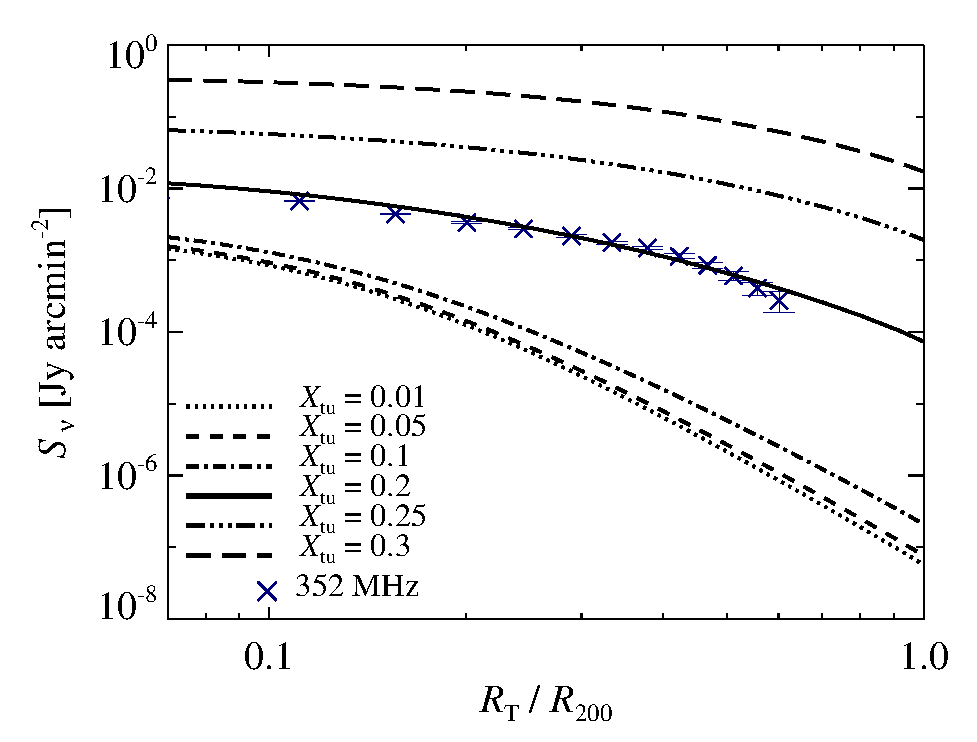
\includegraphics[width=\columnwidth]{prof.comp.KrTTDth.Xtu.eps}
   \end{center}
\end{minipage}
\begin{minipage}{1\columnwidth}
   \begin{center}\Large{radio spectra}\\
     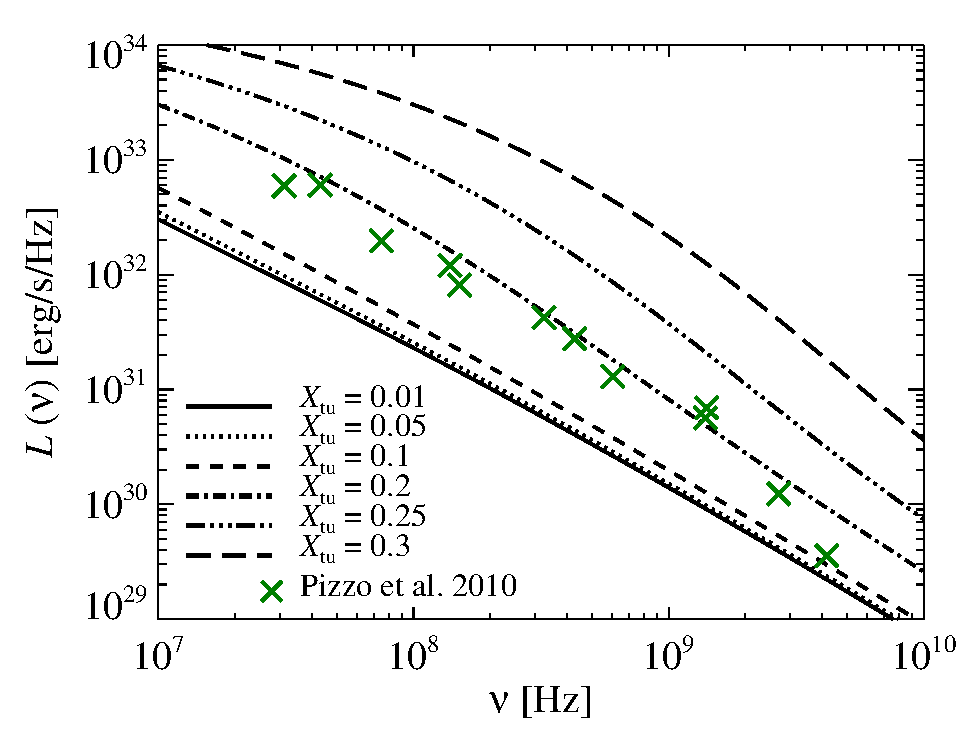
\includegraphics[width=\columnwidth]{spec.comp.KrTTDth.Xtu.eps}
   \end{center}
\end{minipage}
\\
\begin{minipage}{1\columnwidth}
  \begin{center}%\Large{\Mflatturb:}\\ 
    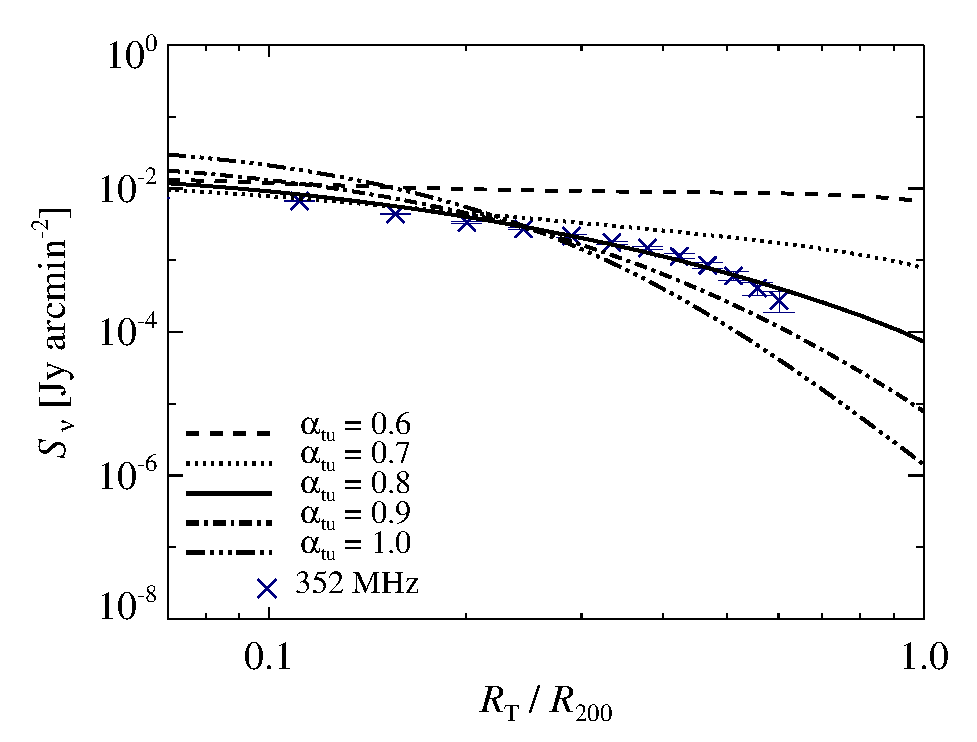
\includegraphics[width=\columnwidth]{prof.comp.KrTTDth.aI0.eps}
  \end{center}
\end{minipage}
\begin{minipage}{1\columnwidth}
   \begin{center}%\Large{\it Brunetti et al. (2012)}:\\
     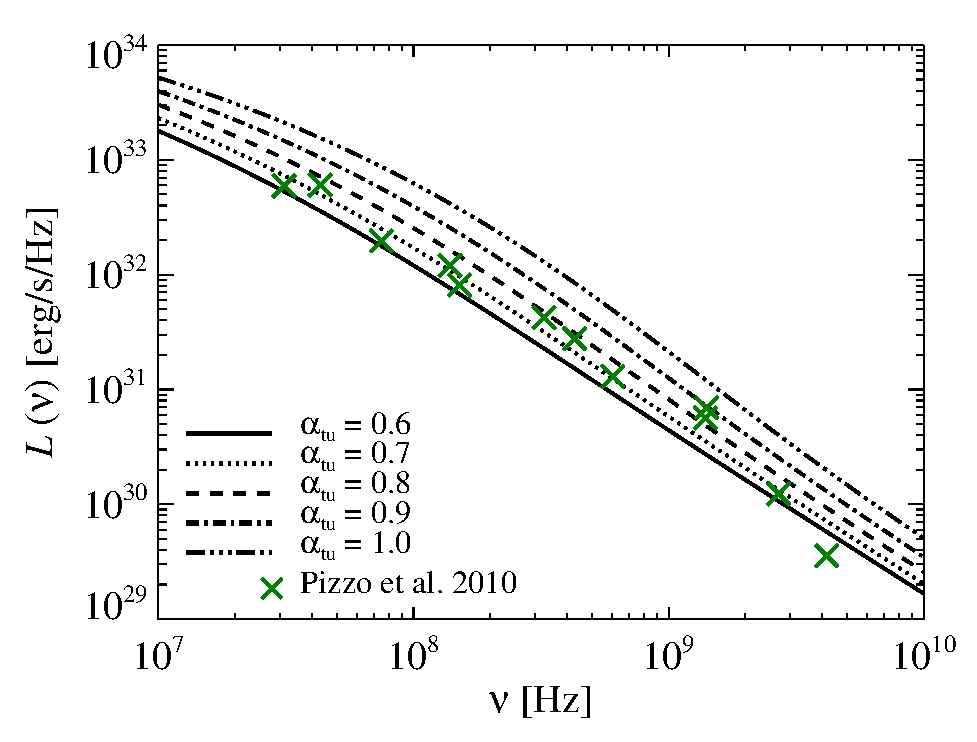
\includegraphics[width=\columnwidth]{spec.comp.KrTTDth.aI0.eps}
   \end{center}
\end{minipage}
\\
\begin{minipage}{1\columnwidth}
  \begin{center}%\Large{\Mflatturb:}\\ 
    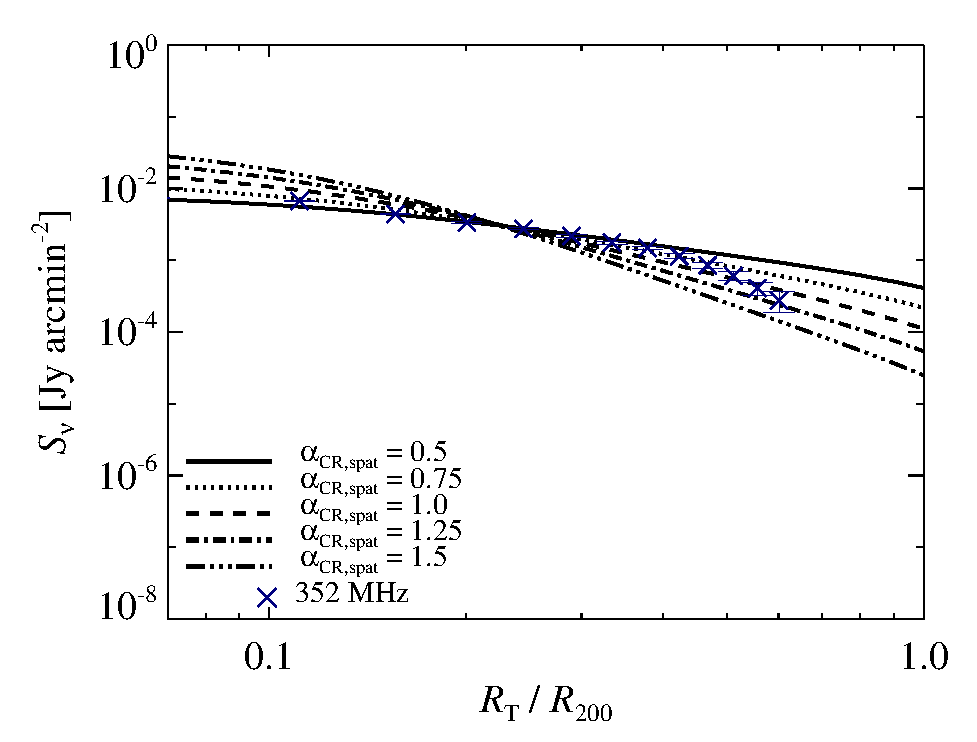
\includegraphics[width=\columnwidth]{prof.comp.KrTTDth.aCR.eps}
  \end{center}
\end{minipage}
\begin{minipage}{1\columnwidth}
   \begin{center}%\Large{\it Brunetti et al. (2012)}:\\
     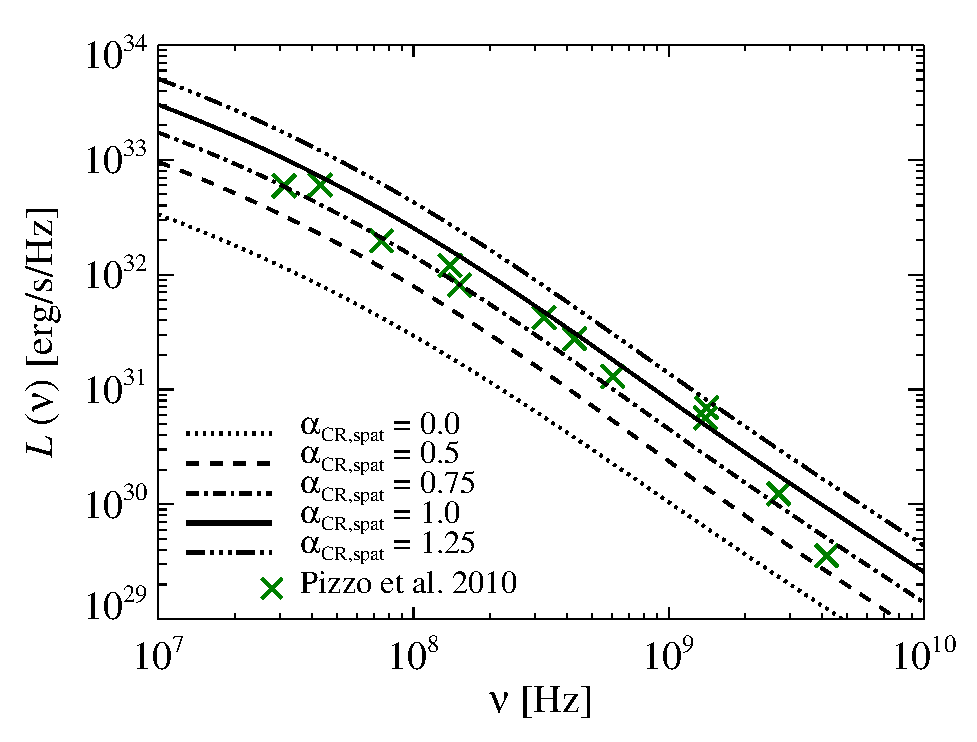
\includegraphics[width=\columnwidth]{spec.comp.KrTTDth.aCR.eps}
   \end{center}
\end{minipage}
\caption{Sensitivity of radio emission in Coma cluster to critical
  parameters. The left-hand panels show the radio surface brightness
  profiles. We compare profiles at 352~MHz \citep[blue
    crosses,][]{brown11} to predicted emission from Fermi-II
  reaccelerated CR electrons populations (black lines). The right-hand
  panels show radio synchrotron spectra. The green crosses are
  compiled from observations \citep{2010PhDT.......259P}, while the
  black lines show predicted emission from reaccelerated CR
  electrons. The upper panels show the sensitivity to the level of
  turbulence ($X_\rmn{tu}$), the middle panels show the impact of
  different turbulent profiles ($\alpha_\rmn{tu}$), and the lower
  panels show the dependence on spatial distributions of initial and
  injected CRs ($\alpha_\rmn{CR,spat}$). We adopt the following
  fiducial values for our model, $X_\rmn{tu}=0.2$,
  $\alpha_\rmn{tu}=0.8$, and $\alpha_\rmn{CR,spat}=1.0$ and vary each
  parameter separately in each row of panels. We find that the radio
  emission is much more sensitive to the level of turbulence while it
  depends less senstively to the spatial distribution of CRs.}
  \label{fig:param_comp}
\end{figure*}


% --- section: Simulation Results and discussion --- %
\section{Cosmological simulations}
\label{sec:results}

In this setion, we solve the Fokker-Planck equation for CR transport
on Lagrangian particle trajectories through cosmic history.  We
concentrate on three scenarios. (i) In model {\em M-primaries}, we
assume that CR electrons, which have been accelerated by cosmic
formation shocks and successively cooled by inverse Compton and
synchrotron losses, form a fossil seed population for
reacceleration. (ii) In model {\em M-streaming}, we account for the
outward streaming of central CRps, which produces a flat CR
distribution in the ICM and equivalently a flat secondary seed
population of CRe for reacceleration. (iii) In model {\em
  M-turbulence} we adopt a spatially flatter turbulent profile than
what was adopted before but assume that seed CRps and secondary CRes
follow the steep profile that is suggested by structure formation
simulations.

The level of emission is mainly driven by how efficient the CRs are
reaccelerated and for how long. Hence, we exploit the exponential
sensitivity of reacceleration on the level of turbulence and adopt
different radial profiles of the turbulent energy density. We ask the
question how differently the turbulent profiles need to be shaped in
order to reproduce the observed radial profiles of the radio
emission. For these models, we then compute radio spectra and
gamma-ray luminosities and compare to observational data.


\subsection{Modelling diffusive shock acceleration}
\label{sec:cosmo_sim}
In this paper we focus on our simulated cluster, g72a, which is a
massive cluster of mass $M_{200}=1.6\times10^{15}\,M_\odot$ that
experienced a merger about 1 Gyr ago
\citep{2009MNRAS.399..497D}. Since the cluster mass, density and
temperature profiles are all similar to the well studied Coma cluster
\citep{2007MNRAS.378..385P,pinzke10}, we will compare our calculations
to radio and gamma-ray observations of Coma.

We use a simple test-particle model for the CR acceleration and
injection, where each shock injects CRs that trace a power-law in
momentum,
\begin{equation}
  f_\p(p,t) = C(t)\,p^{\alpha_\rmn{inj}}\,,\quad
  \alpha_\rmn{inj}=\frac{(\gamma_\rmn{ad}+1)\mathcal{M}^2}
        {(\gamma_\rmn{ad}-1)\mathcal{M}^2+2}
\end{equation}
determined by the normalization $C(t)$ and the spectral index
$\alpha_{\rmn{inj}}$ that depends on the adiabatic index
$\gamma_\rmn{ad} = 5/3$ and the Mach number of the shock
$\mathcal{M}$. It is given by the ratio of the upstream velocity
($\varv_2$) and the sound speed ($c_{\rm s}$). The CR number density and CR
energy density are derived from
\begin{eqnarray}
n_\rmn{p} &=&
\int_{p_\rmn{inj}}^\infty \dd p\, f_\p(p)\\
\eps_\rmn{p} &=&
\int_{p_\rmn{inj}}^\infty \dd p\, f_\p(p) \,E(p),
\end{eqnarray}
where $E(p) = (\sqrt{1+p^2} -1)\, m\,c^2$ is the kinetic energy of a
particle with momentum $p$. We adopt a fit to Monte Carlo simulations
of the thermal leakage process that relates the momentum of injected
protons ($p_\rmn{inj}$) to the thermal energy ($p_\rmn{th}$) of the
shocked plasma \citep{kang11}:
\begin{eqnarray}
  \label{eq:qinj}
  p_\rmn{inj} &=& x_\rmn{inj} p_\rmn{th} = x_\rmn{inj} \sqrt{\frac{2 \,\kB T_2}{m c^2}}\,, \nonumber \\
  \rmn{where}\quad x_\rmn{inj} &\approx& 1.17 \frac{\varv_2}{p_{\rmn{th}}\,c} \left(1+
  \frac{1.07}{\epsilon_B}\right) \left(\frac{\mathcal{M}}{3}\right)^{0.1}\,.
\end{eqnarray}
Here $\eb = B_0/B_{\perp}$, $B_0$ is the amplitude of the downstream
MHD wave turbulence, and $B_{\perp}$ is the magnetic field along the
shock normal. The physical range of $\eb$ is quite uncertain due to
complex plasma interactions. In this paper, we adopt $\eb = 0.23$,
which -- as we will later see -- corresponds to a conservative maximum
energy acceleration efficiency for protons of $10\%$. To derive the
acceleration efficiency, $\zeta_\rmn{inj}$, we first have to infer the
particle injection efficiency, which is the fraction of downstream
thermal gas particles which experience diffusive shock acceleration
\citep[for details see][]{pinzke13},
\begin{equation}
  \label{eq:eta}
  \eta_\rmn{p,lin} =
  \frac{4}{\sqrt{\upi}}\,\frac{x_\rmn{inj}^3}{\alpha_\rmn{inj}-1}\,
  \rmn{e}^{-x_\rmn{inj}^2}.
\end{equation}
The particle injection efficiency is a strong function of
$x_\rmn{inj}$ that depends on both $\mathcal{M}$ and $\eb$. The
energy density of CRs that are injected and accelerated at the shock
(neglecting the CR back reaction on the shock) is given by
\begin{equation}
\label{eq:CR_energy} 
  \Delta\eps_\rmn{p,lin} =
  \eta_\rmn{p,lin}(\mathcal{M})\,n_\rmn{th}(T_2)
  \,\frac{\eps_\p}{n_\p}
\end{equation}
and the CR energy injection and acceleration efficiency is:
\begin{equation}
  \zeta_\rmn{lin} =
  \frac{\Delta\eps_\rmn{p,lin}}{\Delta\eps_\rmn{diss}},
   \quad\mbox{where}\quad
  \Delta\eps_\rmn{diss} = \eps_\rmn{th2} - \eps_\rmn{th0}\,\left(\frac{\rho_2}{\rho_0}\right)^{\gamma_\rmn{ad}}\,.
\label{eqn:energy_frac}  
\end{equation}
The dissipated energy density in the downstream regime,
$\Delta\eps_\rmn{diss}$, is given by the difference of the thermal
energy densities in the pre- and post-shock regimes, corrected for the
adiabatic energy increase due to gas compression.

We limit the acceleration efficiency to $\zeta_\rmn{max}$ by
steepening the spectral index of the injected population
$\alpha_\rmn{inj}$ to $\alpha_\rmn{sub}$ so that $\zeta_\rmn{lin}
\leq \zeta_\rmn{max}$ is always fulfilled. The slope
$\alpha_\rmn{inj}$ impact $\zeta_\rmn{inj}$ via the mean energy per
particle, $\eps_\rmn{p}/n_\rmn{p}$. This
procedure conserves energy and is motivated by models of non-linear
shock acceleration where a sub-shock with a lower compression ratio
(and hence steeper spectral index) forms
\citep[e.g.,][]{2000ApJ...540..292E}. Given our assumed $\eb=0.23$, we
find that for strong shocks where $\alpha \lesssim 2.3$ the spectral
slope is steepened by a maximum of $\sim 10$ per cent in low
temperature regimes ($\kB T\sim 0.1$~keV), while the steepening is much
smaller for high temperature regimes ($\kB T\sim 10$~keV) that are more
relevant for clusters. Since $p_\rmn{inj}$ remains fixed, so does the
CR number density $n_\rmn{p}$. Hence we can solve for the
renormalized normalization constant $C_\rmn{sub}$ using $n_\rmn{p}$
and Eqn.~\ref{eq:eta}:
\begin{equation}
  \label{eq:Cp_sub}
  C_\rmn{sub}=\eta_\rmn{p,lin}\,(\alpha_\rmn{sub}-1)\,p_\rmn{inj}^{\alpha_\rmn{sub}-1}\,,
\end{equation}
where the new distribution function is given by $f_\p(p,t)= C_\rmn{sub}
p^{-\alpha_\rmn{sub}}$. We set an upper limit on the ratio of
accelerated proton-to-dissipated energy in the downstream of strong
shocks that varies from $\zeta_\rmn{max} \sim 1-10\%$, depending on
the adopted model (for more details, see Section \ref{sec:results}).

In our Galaxy, the CRe-to-CRp ratio at a few GeV is $K_{\rmn{ep}} \sim
10^{-2}$. Hence, we adopt this as a fiducial value for the CRe-to-CRp
acceleration efficiency \citep[see][for more
  discussion]{pinzke13}. However, as recent PIC simulations have
shown, this is likely very different at weak shocks, with electrons
efficiently accelerated at perpendicular shocks
\citep{2014ApJ...794..153G,2014ApJ...797...47G}, and ions efficiently
accelerated at parallel shocks \citep{2014ApJ...783...91C}. Thus,
depending on magnetic geometry, $K_{\rmn{ep}}$ could be either larger
or smaller. Some observations of radio relics suggest high values of
$K_{\rmn{ep}}$, due to the absence of gamma-ray emission, which probes
the CRp population \citep{2014MNRAS.437.2291V}. This suggests primary
CRes as a viable alternative scenario to secondary CRes as seeds for
the giant RHs. In our {\em M-primaries} scenario, the injected
distribution of CRes is derived in the same way as for the CRps. Once
they have been accelerated to relativistic energies, injected
electrons and protons are indistinguishable. We therefore assume that
CRp and CRe have the same distribution function $f_\rmn{e}(p) =
K_\rmn{ep} f_\rmn{p}(p)$, with a different normalization (due to
differing acceleration efficiencies) $K_\rmn{ep}=0.1$ \citep[which is
  viable for primarily perpendicular
  shocks,][]{2014ApJ...794..153G}. While this appears to contradict the
radial bias of magnetic fields in the bulk of the ICM as suggested by
observations \citep{2010NatPh...6..520P} and cluster simulations
\citep{2011ApJ...740...81R}, it does not necessarily apply to the
accretion shock regions, which show a field geometry with a net
perpendicular bias with respect to the shock normal---at least for
giant radio relics \citep{2010Sci...330..347V}.


\subsection{Radio emission profile}

\begin{figure*}
\begin{minipage}{1\columnwidth}
   \begin{center}\Large{\Mprimary:}\\
     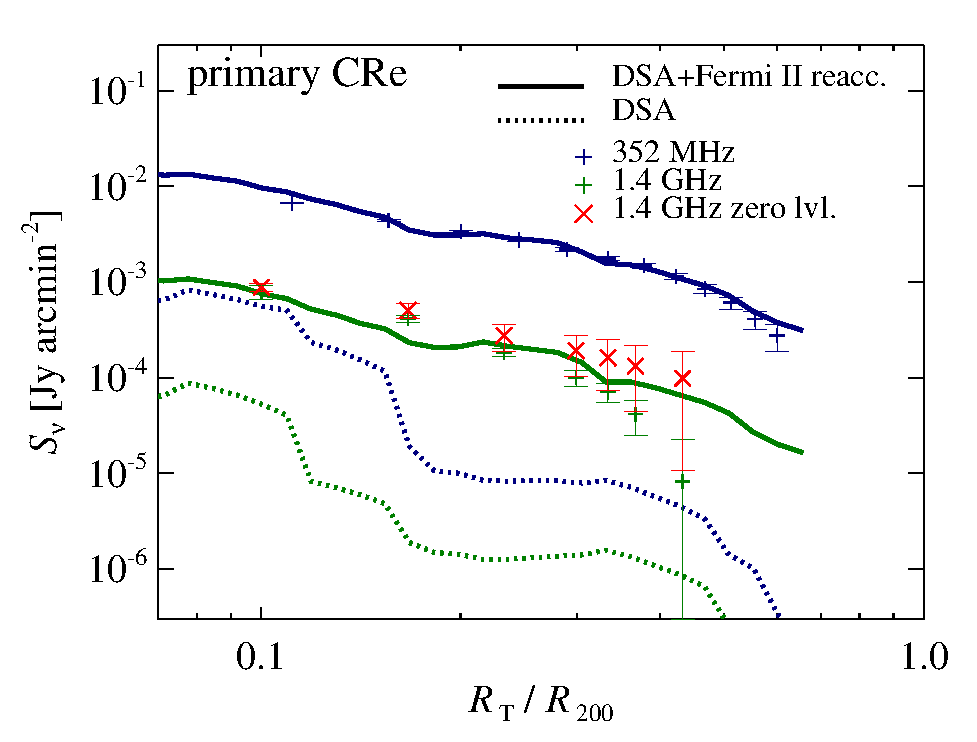
\includegraphics[width=\columnwidth]{sbright.nu.DIIcomp.Pri.g72a.Rad14.2400p.z0.NL.xKR.eb23.eI088.140.v6.eps}
   \end{center}
\end{minipage}
\begin{minipage}{1\columnwidth}
   \begin{center}\Large{\Mstream:}\\
     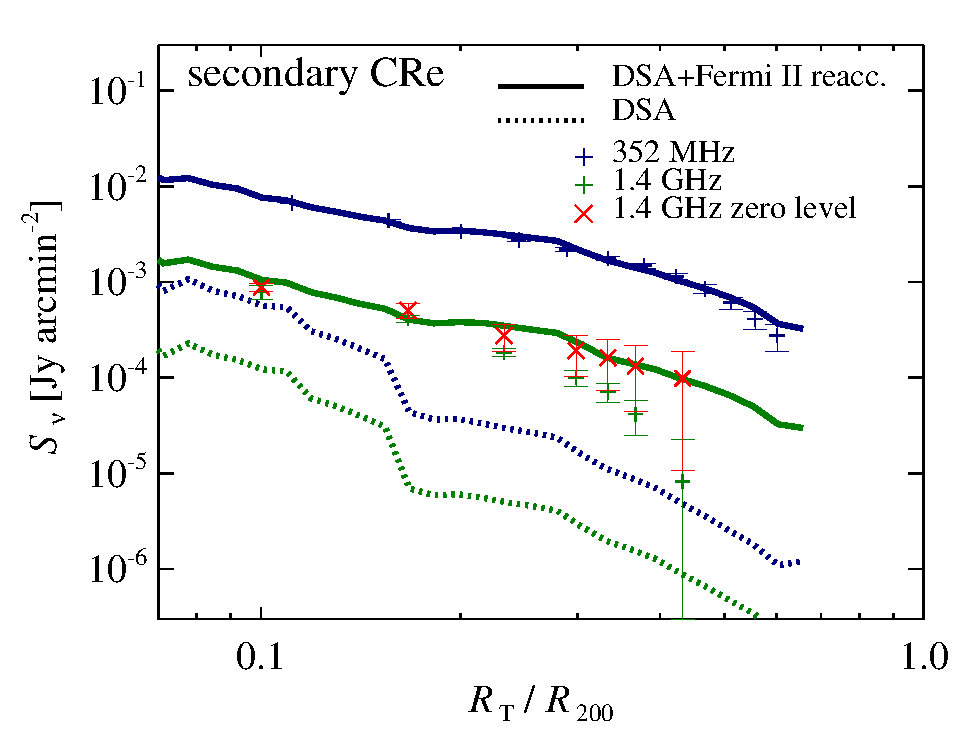
\includegraphics[width=\columnwidth]{sbright.nu.DIIcomp.flatCR.g72a.Rad14.2400p.z0.NL.xKR.eb23.eI082.flatCR.140.v6.eps}
   \end{center}
\end{minipage}
\\
\begin{minipage}{1\columnwidth}
  \begin{center}\Large{\Mflatturb:}\\ 
    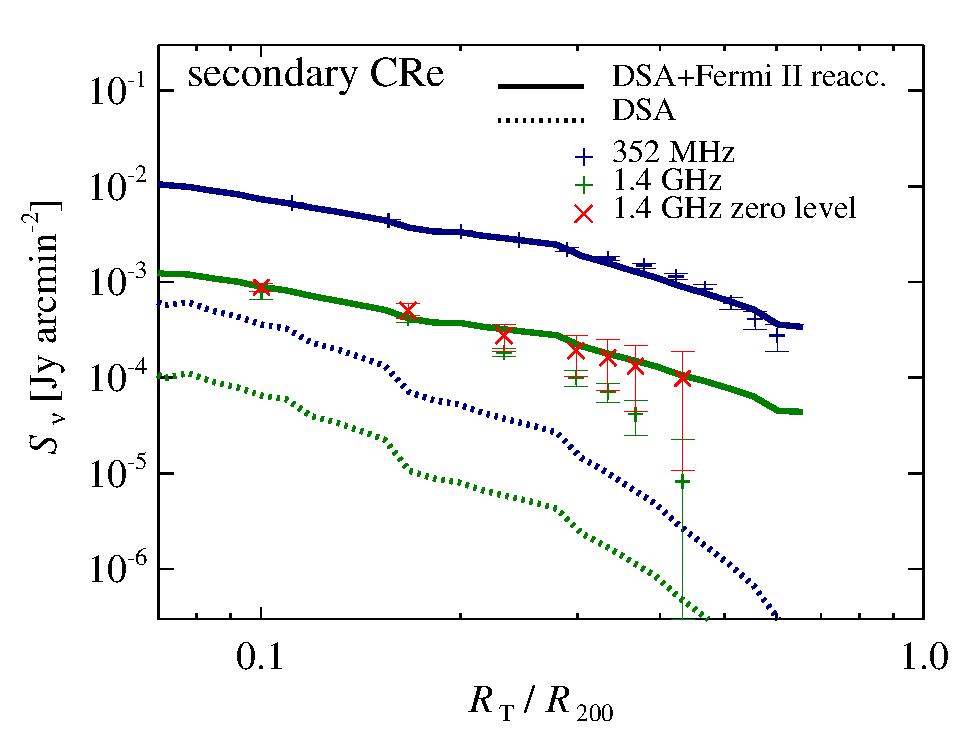
\includegraphics[width=\columnwidth]{sbright.nu.DIIcomp.I0.g72a.Rad14.2400p.z0.NL.xKR.eb23.eI067.140.v6.eps}
  \end{center}
\end{minipage}
\begin{minipage}{1\columnwidth}
   \begin{center}\Large{\it Brunetti et al. (2012)}:\\
     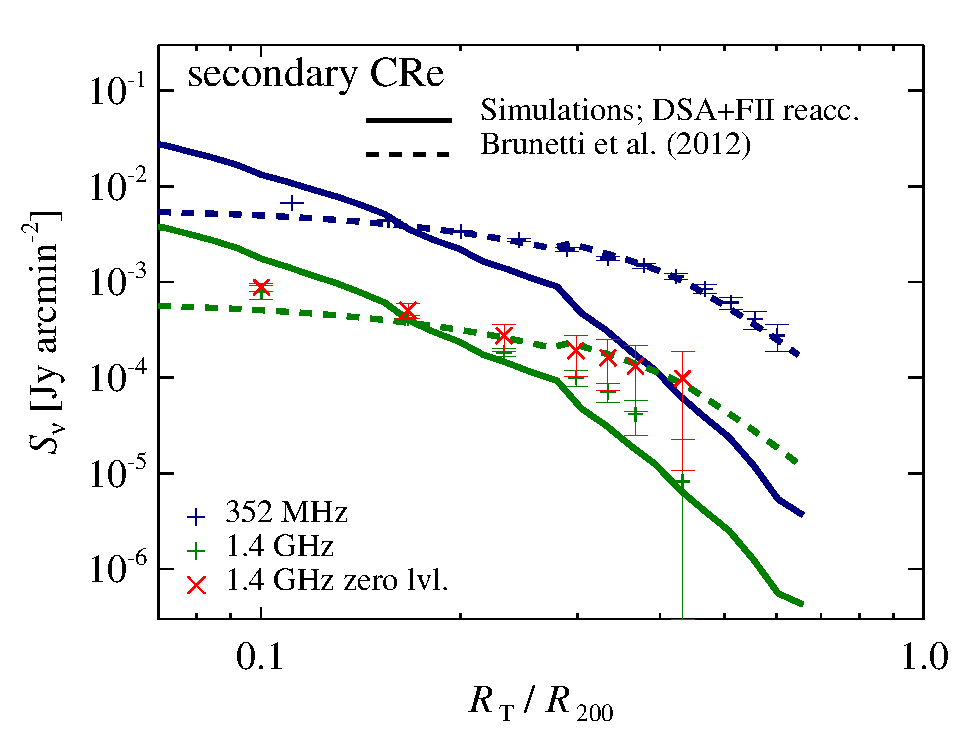
\includegraphics[width=\columnwidth]{sbright.nu.DIIcomp.Brunetti.g72a.Rad14.2400p.z0.NL.xKR.eb23.140.v6.eps}
   \end{center}
\end{minipage}
\caption{Radio surface brightness profiles of Fermi-II reaccelerated
  CR electrons of a simulated post-merging cluster similar to Coma. We
  compare profiles at 352~MHz \citep[blue lines and
    crosses,][]{brown11} to those at 1.4~GHz \citep[green lines and
    crosses,][]{deiss97}. The red crosses show the reprocessed 1.4~GHz
  data, where a zero level of about 10~\% of the central value is
  adopted. The solid lines show predicted emission from a
  reaccelerated fossil population, while dotted lines show emission
  from a fossil population without reacceleration. The panels show the
  emission of our models \Mprimary (upper left panel), \Mstream (upper
  right panel), \Mflatturb (lower left panel), and simulated secondary
  electrons together with previous estimates \citep{brunetti12} for
  the Coma cluster (lower right panel).}
  \label{fig:sync_profile}
\end{figure*}

In Fig.~\ref{fig:sync_profile}, we show radial profiles for the radio
emission in all three scenarios in which the seeds undergo Fermi-II
reacceleration in turbulent fields that are shaped such as to
reproduce the Coma RH profile at 352~MHz.  Adopting our
parametrisation for the volumetric injection rate of turbulent energy,
$I_0\propto \eps_\rmn{th}^{\alpha_\rmn{tu}}$, we find
$\alpha_\rmn{tu}= 0.67$ for \Mflatturb, $\alpha_\rmn{tu}= 0.82$ for
\Mstream, and $\alpha_\rmn{tu}= 0.88$ for \Mprimary. As a result, the
ratio of turbulent-to-thermal energy densities slightly increase with
radius as shown in Fig.~\ref{fig:turb}.  After turbulent
reacceleration, the volume-weighted, relative CRp energy density and
relative CRp number density inside the RH for \Mflatturb (\Mstream),
are found to be 2 (3) \% and $2\times10^{-8}$ ($5\times10^{-8}$),
respectively.

%the turbulent energy density becomes $\eps_\rmn{turb} \propto
%\eps_\rmn{th}^{(\alpha_\rmn{tu}+1)/2}/T^{1/4}$, where $T$ is the
%temperature of the gas,

\begin{figure}
  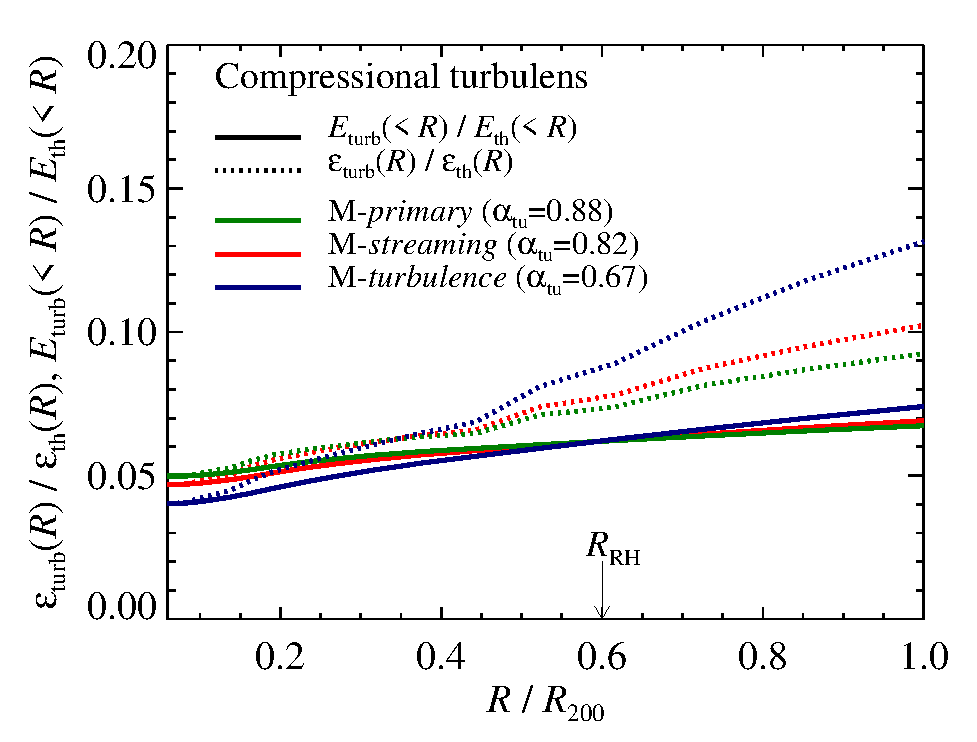
\includegraphics[width=1.0\columnwidth]{turb_profile_ratio_tot.eps}
  \caption{The ratio of turbulent-to-thermal energy densities (solid
    lines) and cumulative energies (dotted lines) in our three
    models. The energy densities are parametrized as
    $\eps_\rmn{turb} \propto
    \eps_\rmn{th}^{(\alpha_{\rmn{tu}}+1)/2}/T^{1/4}$ and
    normalized such that the total turbulent energy in compressible
    modes $E_\rmn{turb}$ for each scenario makes up about 20\% of the
    total thermal energy $E_\rmn{th}$ inside the radio halo
    ($R_\rmn{RH}\approx0.6R_{200}$). The turbulent profiles explore
    the uncertainty in the cluster turbulence and are motivated by the
    cosmological simulation in
    \citep{2009ApJ...705.1129L,2010ApJ...725.1452S,2011A&A...529A..17V}.}
  \label{fig:turb}
\end{figure}

Figure~\ref{fig:sync_profile} demonstrates that the modeled radio
profiles without turbulent reacceleration are too steep.  In the
bottom right panel of Fig.~\ref{fig:sync_profile} (labeled with
Brunetti et al. 2012), we show that our simulated profiles of
reaccelerated CRs, which only take advective CR transport into
account, i.e. they neglect CR streaming or a flatter turbulent
profile, produce radio profiles that are too steep. Indeed, even using
the assumptions of previous work -- where complete freedom in the seed
population was allowed -- it is not possible to reproduce observations
in both frequencies in any model.\footnote{Note that in previous work
  on the Coma cluster, $\eps_\rmn{turb} \propto \eps_\rmn{th}$ was
  adopted which approximately corresponds to $\alpha_\rmn{tu}= 1$
  \citep{brunetti12} and together with the different distributions for
  seed CRes constitute the main differences compared to our work.}
Decreasing the acceleration efficiency with radius does not change
this conclusion much because of the weak radial dependence of
$D_\rmn{pp}(R)\propto \eps_\rmn{th}(R)^{\alpha_\rmn{tu}-1}
\sqrt{T(R)}$. This signals that the problem is generic and requires
either additional modifications to the plasma physics of acceleration
or a better understanding of potential observational systematics. In
addition there are differences in the simulated density and
temperature profiles in comparison to the observed profile in Coma
that impact the CR abundance as well as cooling and reacceleration.

In Figure~\ref{fig:tauD} we show how the turbulent reacceleration
timescales in our three models scale with radius. As expected, the
\Mprimary model with $\alpha_\rmn{tu}=0.88$ has the flattest profile
with $\tau_D\approx0.4\,\rmn{Gyr}$, where the small dip at large
radius driven by the decrease in thermal energy density. The
\Mflatturb model has the the flattest turbulent profile parameterized
by the smaller $\alpha_\rmn{tu}$ which explains the steepest $\tau_D$
profile. Note that a fixed reacceleration timescale is required to
explain the observations at each radius and for each model (see also
Table~\ref{tab:timescales}). This allows us to interchange the value
of uncertain parameters $\tau_\rmn{cl} \sim X_\rmn{tu}^2 \sim k_0$,
i.e. a longer reacceleration duration have to be compensated by
lowering the level of turbulence or increasing the physical injection
scale of turbulence to keep $\tau_D$ constant.

\begin{figure}
  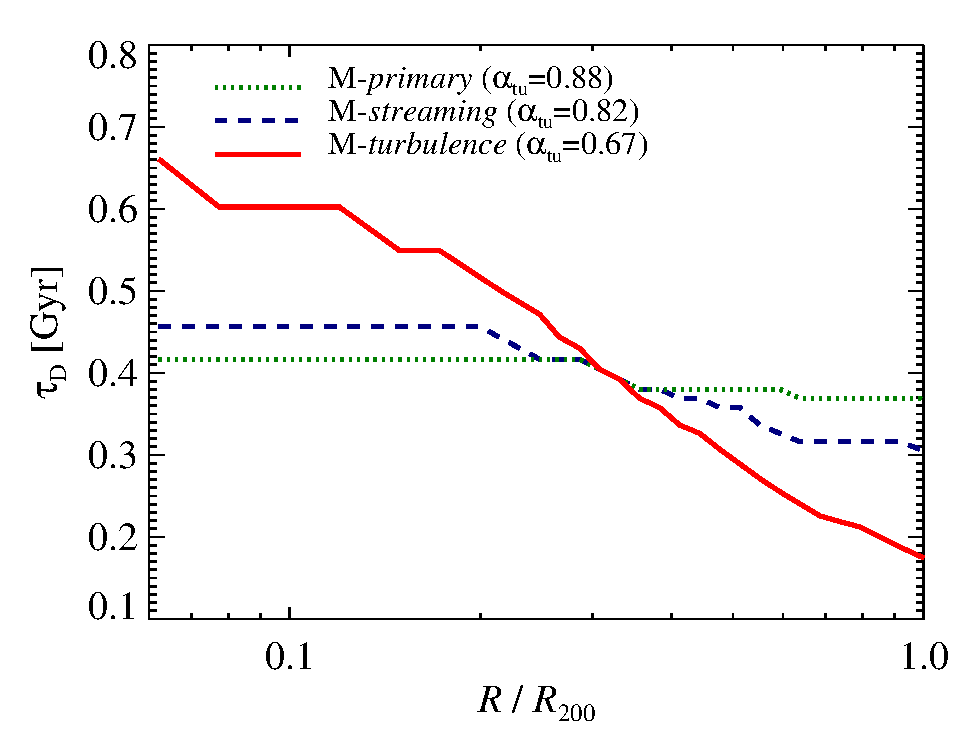
\includegraphics[width=1.0\columnwidth]{tau_reacc.eps}
  \caption{Turbulent reacceleration timescales for our simulated
    cluster g72a. We show in linear-log the reacceleration timescale
    ($\tau_D$) as a function of radius $R$ for our three models:
    \Mprimary (green dotted line), \Mstream (blue dashed line), and
    \Mflatturb (red solid line). Note that the timescales are derived
    during the last 100~Myrs in time in our simulations.}
  \label{fig:tauD}
\end{figure}

In principle, reacceleration via TTD leads to spectral steepening with
particle energy due to the inefficiency of the acceleration process to
counter the stronger cooling losses with increasing energy. Since
synchrotron emission peaks at frequency $\nu_\rmn{syn}\simeq 1\,
B/\umu\rmn{G} (\gamma/10^4)^2\,\rmn{GHz}$, this translates into a
spectral steepening of the radio spectrum (see the left panel of
Fig.~\ref{fig:sync_spectrum} where the continuous injection of
secondary CRes is absent). A given radio window samples higher energy
electrons for a decreasing field strength in the cluster
outskirts. Hence, the spectral steepening with energy should translate
into a radial spectral steepening \citep{brunetti12}. However, because
of the weak dependence of the electron Lorentz factor on emission
frequency ($\gamma\propto\sqrt{\nu_\rmn{syn}}$), this effect is only
visible in our simulations for $\nu_\rmn{syn}\gtrsim5$~GHz. Most
importantly, our simulated fluid elements at a given radius sample a
broad distribution of shock history, density and temperature, which
implies very similar synchrotron brightness profiles at
$\nu_\rmn{syn}=352$~MHz and 1.4 GHz. The discrepancy of the observed
and simulated 1.4 GHz profiles could instead be due to systematic flux
calibration error in single dish observations. These could arise, for
instance, due to errors in point source subtraction. Interestingly, we
can match the 1.4 GHz data if we reduce the zero point by adding 10\%
of the central flux to every data point; this flattens the outer
profile\footnote{Lawrence Rudnick, private communication.}.
Alternatively, this may point to weaknesses in the theoretical
modeling of the particle acceleration process and may require a
stronger cutoff in the particle energy spectrum.


\subsection{Radio spectrum}
\label{sect:radio_spec}
In Fig.~\ref{fig:sync_spectrum} we show that our three models that
include Fermi-II reacceleration can individually reproduce the
convexly curved total radio spectrum found in the Coma cluster. Seed
CRs in \Mstream and \Mflatturb that do not experience turbulent
reacceleration have a power-law spectrum in disagreement with
observations. In order to match both the spatial and spectral profiles
in Coma, we adopt an acceleration efficiency for the strongest shocks
in our three models \Mprimary, \Mstream, and \Mflatturb to
$\zeta_{\rmn{e}} <0.003$, $\zeta_{\rmn{p}} < 0.1$, and
$\zeta_{\rmn{p}}<0.03$, respectively. Following the Mach number
($\mathcal{M}$)-dependence of the acceleration efficiency suggested in
\cite{pinzke13}, the efficiency in weak shocks ($\mathcal{M}\sim
2.5-3.5$) that dominates the CR distribution function, has an
acceleration efficiency for protons $\zeta_{\rmn{p}}\sim0.0001-0.01$,
and for electrons $\zeta_{\rmn{e}}\sim 0.001$.

Interestingly, we find that the radio luminosity from clusters in the
OFF-state (DSA only) and ON-state (DSA and reacceleration) differ by
about a factor 10-20 in all our three models. This means that the
secondary CRes are dominated by the reaccelerated fossil CRes and not
from the CRes produced by reaccelerated CRps. However, for high
frequencies ($\nu_\rmn{syn}\gtrsim$ GHz) where synchrotron cooling is
more efficient than reacceleration, the emission is dominated by the
CRes produced in the continuous injection of electrons from
reaccelerated CRps. It is also worth mentioning that the radio
emission from secondary CRes are smoothly distributed around the
cluster because of the continuous injection, hence the it is not
dominated by outliers.

However, for \Mprimary, the primary CRes that generate most of the
radio emission from the cluster in the OFF-state are dominated by only
a small fraction of the CRes. These electrons are injected very
recently and have not had time to cool yet. Hence we expect there to
be a large variance in the OFF-state of different simulated
clusters. As mentioned in section~\ref{sect:param_comp}, combining
radio observations with gamma-ray limits allows us to put a lower
limit to $X_\rmn{tu}$.  If $X_\rmn{tu}$ is smaller than in our adopted
models (where we assume $X_\rmn{tu}=0.2$), then the efficiency of DSA
has to be larger than $\zeta_\rmn{p}\sim 0.1$ for the secondary CRes
to reproduce the radio observations. However, since the turbulent
reacceleration acts on both the secondary CRes and the CRps, while
$\zeta_\rmn{p}$ only affects the CRps, \Mstream and \Mflatturb would
produce too much gamma-rays. Hence we conclude that
$X_\rmn{tu}\gtrsim0.2$ if all other parameters are kept
fixed. Although, we caution the reader to take this limit too
stringent because of the uncertainty in $k_0$ and $\tau_\rmn{cl}$ that
impact $X_\rmn{tu}$ for a fixed $\tau_\rmn{D}$. This parameter space
needs to be explored further in future work in order to put more
stringent limits on the level of turbulence in clusters using radio
and gamma-ray observations in combination with turbulent reaccelerated
CRs.

\begin{figure*}
  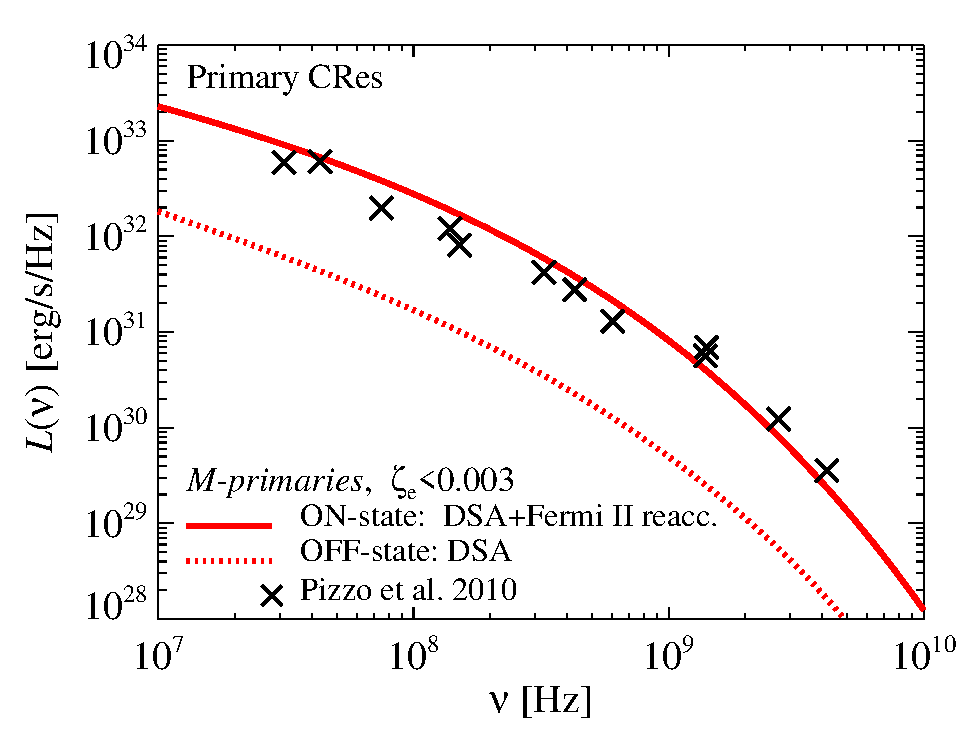
\includegraphics[width=1.0\columnwidth]{sync.spec.pri.g72a.140.v6.eps}
  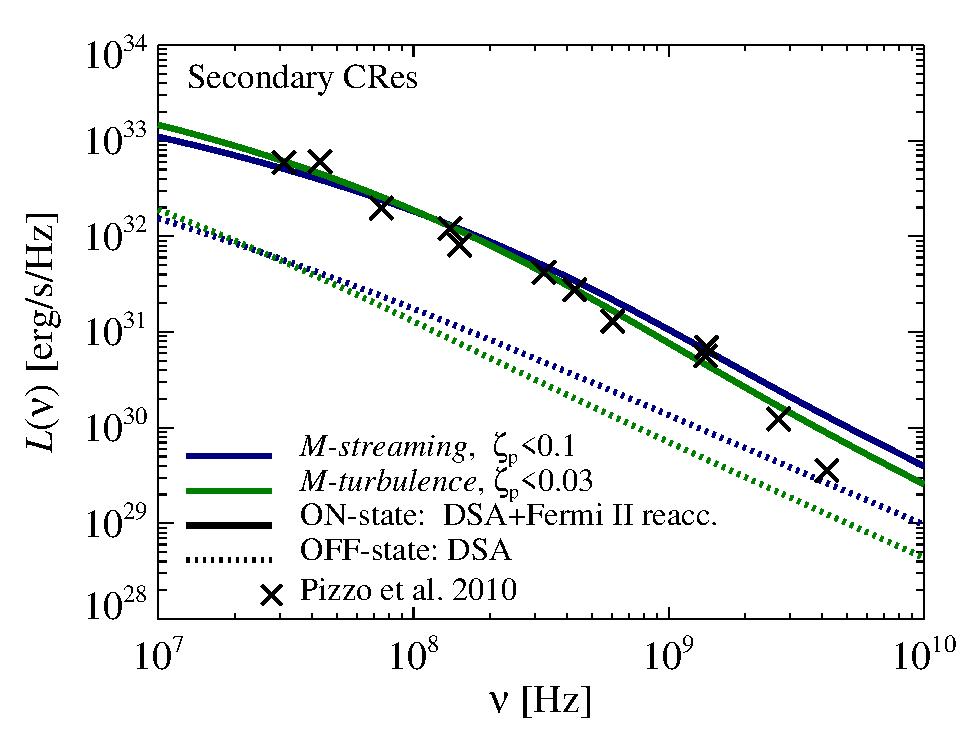
\includegraphics[width=1.0\columnwidth]{sync.spec.sec.g72a.140.v6.eps}
  \caption{Radio synchrotron spectra. Lines are derived from
    simulations, while the black crosses are compiled from
    observations \citet{2010PhDT.......259P}. The solid lines show the
    DSA and reaccelerated CRs (On-state of the radio halo), while the
    dotted lines show CRs accelerated only by DSA (Off-state of the
    radio halo). The left figure shows the radio emission induced by
    primary CRes and the right figure shows the emission from
    secondary CRes. The different line colors represent our different
    models, \Mprimary (red line), \Mstream (blue line), and \Mflatturb
    (green line).}
  \label{fig:sync_spectrum}
\end{figure*}

\subsection{Gamma rays}
The gamma-ray emission from CRps that produce decaying neutral pions
could be substantial if the CRps are reaccelerated efficiently enough,
hence it is interesting to estimate this emission for our models and
compare to upper limits. \AP{We follow the formalism outlined in
  \cite{1999APh....12..169B} (and references therein) and calculate
  the gamma-ray emission numerically for our three models.} We predict
the gamma-ray emission from \Mflatturb (\Mstream) with
$F_\gamma(>500\,\rmn{MeV})=4\times10^{-10} (5\times10^{-10}) \mathrm{
  \,ph\, s}^{-1}\mathrm{cm}^{-2}$. The fluxes from these models are
slightly larger than in \cite{brunetti12}, where the differences comes
from our steeper CRp profiles in addition to simulation based
formalism we rely on that accounts for both Coulomb and hadronic
losses during the build up of the CR distribution in contrast to the
scaling relations adopted in their paper. Interestingly the gamma-ray
flux from both our scenarios are just below recent Fermi-LAT limits
derived from a gamma-ray profile similar to \Mflatturb where
$F_\gamma(>500\,\rmn{MeV})<5.3\times10^{-10} \mathrm{ \,ph\,
  s}^{-1}\mathrm{cm}^{-2}$ \footnote{Fabio Zandanel, private
  communication. See also
  \citet{2014MNRAS.440..663Z,2014ApJ...787...18A}. and will be probed
  in the next few years by Fermi-LAT. } The spectral index of the CRp
distribution is relatively steep ($\alpha_{\rmn{p}}\sim2.6$) for the
CRp energies $E \gtrsim 10$~GeV that are relevant for the injection of
radio-emitting secondary CRes. The steep spectrum is ultimately a
consequence of the shock history of the simulated cluster, with a weak
dependence on our test particle model for Fermi-I acceleration
\citep{pinzke13}, where we steepen the spectral index to avoid
acceleration efficiencies above $\zeta_{\rmn{p}} \sim 10\%$.


% --- section: Conclusions --- %
\section{Conclusions}
\label{sec:conclusions}

The standard reacceleration model for radio halos (RHs) requires a
population of seed electrons to undergo turbulent
reacceleration. These seeds are generally thought to be secondary
electrons from hadronic cosmic ray proton (CRp) interactions. In this
work we use cosmological simulations to derive a population of seed CR
protons originating from structure formation shocks and merger shocks
during the cluster build up. The resulting secondary population is
inconsistent with RH observations. We propose three possible solutions
where all reaccelerated CRs produce gamma-ray emission below current
upper limits. Additionally, they reproduce both the spectrum and the
surface brightness profiles of the Coma radio halo:

\begin{enumerate}
\item {\bf Model {\em M-primaries}.} If indeed the acceleration
  efficiency of CRps is below about $0.1$ {\%} in weak shocks and the
  ratio of injected electrons and protons is $K_{\rmn{ep}} \sim
  10^{-1}$, CR electrons accelerated directly in shocks dominate over
  secondaries.
\item {\bf Model {\em M-streaming}.} Alternatively, CRps could stream
  out of the central core and produce flat CR profiles. This seed
  population of secondary CRes also has the correct spatial and
  spectral features alone, or potentially complements primaries to
  explain radio observations.
\item {\bf Model {\em M-turbulence}.}  Finally, injected turbulence
  that is flatter than in previously adopted models, which allows seed
  CRps to follow the steep radial profile that is suggested by
  structure formation simulations.
\end{enumerate}

Combining radio observations with gamma-ray constraints can be very
useful to learn about the plasma of the intracluster medium. Our
models (ii) and (iii) relies on CRps to induce secondary CRes that
produce the observed radio emission. In addition proton-proton
collisions produce neutral pions that decay into gamma rays. Since
turbulent reacceleration acts on both CRes and CRps, while the DSA
acceleration efficiency ($\zeta_p$) only acts on the CRps, radio
observations fix the relation between $X_\rmn{tu}$ (the ratio of the
total turbulent energy in compressional modes to the total thermal
energy) and the acceleration efficiency. With the addition of
gamma-ray constraints from Fermi-LAT, we can derive a lower limit to
$X_\rmn{tu}\gtrsim0.2$ and a upper limit to the acceleration
efficiencies of $\zeta_p\lesssim 10\%$ ($\zeta_p\lesssim 3\%$) for
the two models, respectively, for our current choices of other
parameters.

How could we distinguish the different possibilities of a dominating
primary or secondary seed population of electrons observationally?
One possibility that is relative insensitive to adopted parameters in
our models is to use high-frequency radio observations (with e.g., the
Jansky Very Large Array) where turbulent reacceleration of CRes (which
has a high energy cutoff) is no longer efficient since their fast
radiative cooling time drops below the comparably slow reacceleration
timescale producing a sharp spectral cutoff. This is unlike
reacceleration of CRps that do not suffer radiative cooling losses and
inject power-law momentum distributions of secondary CRe (see
Fig.~\ref{fig:sync_spectrum}).

However, the negative flux bowl of the Sunyaev-Zel'dovich effect
introduces a cutoff of the RH spectrum at frequencies above $\gtrsim
10$~GHz \citep[][ depending on cluster mass and
  redshift]{2002A&A...396L..17E,Pfrommer:2003mk}. Hence the
subdominant radio emission from freshly injected secondary CRes may
only be detectable in steep spectrum radio sources
\citep{2008Natur.455..944B}, which exhibit a cutoff at lower radio
frequencies and are thought to represent dying RHs as a result of the
decaying turbulence after a merger. Alternatively, one could attempt
to reconstruct the intrinsic high-frequency RH spectrum by filling in
the missing flux due to the Sunyaev-Zel'dovich effect by precise
measurements of the Compton-$y$ parameter at microwave
frequencies. Another possibility would consist in stacking the radio
data of radio-quiet clusters that do not exhibit RH emission
individually \citep{2011ApJ...740L..28B}. This may reveal the
glow of radio emission due to steady state secondary
population. Emission from faint secondary electrons should still be
visible, whereas due to the much more intermittent nature of DSA
injection, primary CRe will instead show a sharp cutoff due to
cooling, and will not be visible at high energies (see
Fig.~\ref{fig:sync_spectrum}).

As MHD simulations of clusters that follow spectral CR distributions
become feasible, these will provide valuable insight about the profile
and the total energy of turbulence in clusters and the possibility of
turbulent reacceleration. This will further help us to distinguish the
three different models from each other. We will pursue further
implications and distinguishing characteristics of these competing
models in future work.


{\bf Acknowledgments.} We thank Josh Wiener for discussions on CR
streaming. We are also grateful to Lawrence Rudnick for discussion on
uncertainties in the 1.4 GHz radio data. Finally, we thank Fabio
Zandanel for recalculating gamma-ray limits and Gianfranco Brunetti
for useful discussions. A.P. is grateful to the Swedish research
council for financial support. S.P.O. thanks NASA grant NNX12AG73G for
support. C.P.~acknowledges support by the European Research Council
under ERC-CoG grant CRAGSMAN-646955 and by the Klaus Tschira
Foundation.


%%%%%%%%%%%%%%%%%%%%%%%%%%%%%%%%%%%%%%%%%%%%%%%%%%%%%%%%%%%%%%%
\vspace{-0.7cm}

\bibliography{paper}
\bibliographystyle{mnras}

\end{document}
